%:\documentclass[cjk,slidestop,compress,mathserif,blue]{beamer}
\documentclass[cjk,slidestop,handout,compress,mathserif,blue]{beamer}	%打印PPT用,handout(讲义)可去掉过渡效果,如\pause引起的多页显示,为打印时节省纸张
%dvipdfm选项是关键,否则编译统统通不过
%beamer的颜色选项定义的是导航条和标题的颜色(即关键词structure的颜色)

%%%%%%%%%%%%%%%%仅限于XeTeX可使用的宏包%%%%%%%%%%%%%%%%%%%%%%%%%%%%
\usepackage{fontspec,xunicode,xltxtra,beamerthemesplit}
%\usepackage{beamerthemesplit}
\usepackage{xeCJK}
\setCJKmainfont[BoldFont=黑体, ItalicFont=楷体, BoldItalicFont=仿宋]{黑体}
%\setsansfont[Mapping=tex-text]{Adobe 黑体 Std}
%如果装了Adobe Acrobat,可在font.conf中配置Adobe字体的路径以使用其中文字体
%也可直接使用系统中的中文字体如SimSun,SimHei,微软雅黑 等
%原来beamer用的字体是sans family;注意Mapping的大小写,不能写错

%%%%%%%%   确定标题和导航条结构的框架     %%%%%%%%%%%%
\usepackage{beamerthemeshadow}                       %
%\usepackage{beamerthemeclassic}%导航条色与背景色一致%
%%%%%%%%%%%%%%%%%%%%%%%%%%%%%%%%%%%%%%%%%%%%%%%%%%%%%%
\setbeamerfont{roman title}{size={}}
%\usepackage{CJK} % CJK 中文支持                                  %
\usepackage{amsmath,amsthm,amsfonts,amssymb,bm}
\usepackage{mathrsfs}
\usepackage{xcolor}                                        %使用默认允许使用颜色
\usepackage{hyperref} 
\usepackage{graphicx}
\usepackage{subfigure}           %图片跨页

%\usepackage[numbers,sort&compress]{natbib} %紧密排列             %
\usepackage[sectionbib]{chapterbib}        %每章节单独参考文献   %
\usepackage{hypernat}                                                                         %
%\usepackage[dvipdfm,bookmarksopen=true,pdfstartview=FitH,CJKbookmarks]{hyperref}		%
\hypersetup{bookmarksnumbered,colorlinks,linkcolor=brown,citecolor=blue,urlcolor=red}         %
%参考文献含有超链接引用时需要下列宏包,注意与natbib有冲突        %
%\usepackage[dvipdfm]{hyperref}                                  %
%\usepackage{hypernat}                                           %
\newcommand{\upcite}[1]{\hspace{0ex}\textsuperscript{\cite{#1}}} %

%\useoutertheme{smoothbars}
\useinnertheme[shadow=true]{rounded}
\usetheme{Berkeley}                                          %主题式样
%\usetheme{Luebeck}

\usecolortheme{lily}                                        %颜色主题式样

\usefonttheme{professionalfonts}                           %字体主题样式宏包

%\beamertemplatetransparentcoveredhigh                      %使所有被隐藏的文本高度透明
\beamertemplatetransparentcovereddynamicmedium             %使所有被隐藏的文本完全透明,动态,动态的范围很小
\mode<presentation>
%\beamersetaveragebackground{gray}                          %设置背景颜色(单一色) 
\beamertemplateshadingbackground{green!10}{red!5}         %设置背景颜色(渐变色)

%在指定位置精确放置logo
\usepackage{tikz}
\usepackage{beamerfoils}
\usepackage{pgf}
\logo{\pgfputat{\pgfxy(11.68,0.15)}{
\includegraphics[height=1.01cm,viewport=0 0 140 120,clip]{Figures/BCC_logo-1.png}}\pgfputat{\pgfxy(10.502,-0.218)}{
\includegraphics[height=0.369cm,viewport=140 0 540 120,clip]{Figures/BCC_logo-1.png}}}
%\logo{\pgfputat{\pgfxy(11.68,0.15)}{
\includegraphics[height=0.95cm,viewport=0 0 510 360,clip]{Figures/Logo_Gainstrong.png}}\pgfputat{\pgfxy(10.333,-0.195)}{
\includegraphics[height=0.35cm,viewport=530 70 1100 218,clip]{Figures/Logo_Gainstrong.png}}}
%\MyLogo{
%	\pgfputat{\pgfxy(-50,-50)}{\pgfbox[right,base]{
\includegraphics[height=1cm]{Figures/BCC_logo-1.png}}}
%logo作为背景放置
%\setbeamertemplate{background}{
%	\pgfputat{\pgfxy(6.5,-0.5)}{\pgfbox[left,top]{\pgfimage[height=1.1cm]{Figures/BCC_logo-1.png}}}}

%\logo{}									%不显示logo

\begin{document}
%\begin{CJK*}{GBK}{song}
%\begin{CJK*}{GBK}{kai}
%beamer下不能用\songyi、\zihao等命令!
%\graphicspath{Figures/}

%-------------------------------PPT Title-------------------------------------
\title{课题一任务进展}
%-----------------------------------------------------------------------------

%----------------------------Author & Date------------------------------------
\author[Jiang]{姜\;\;骏\inst{}} %[]{} (optional, use only with lots of authors)
% - Give the names in the same order as the appear in the paper.
% - Use the \inst{?} command only if the authors have different
%   affiliation.
\institute[BCC]{\inst{}%
 \vskip -5pt 北京市计算中心}
\date[\today] % (optional, should be abbreviation of conference name)
{
{\fontsize{6.2pt}{3.2pt}\selectfont{\textcolor{blue}{E-mail:~}\url{jiangjun@bcc.ac.cn}}}
%\vskip 30pt {\fontsize{6.2pt}{3.2pt}\selectfont{清华大学\;\;物理系}}
\vskip 35pt {\fontsize{8.2pt}{6.2pt}\selectfont{上海}}
\vskip 5pt {\fontsize{7.2pt}{3.2pt}\selectfont{2019.~06}}
}

% - Either use conference name or its abbreviation
% - Not really information to the audience, more for people (including
%   yourself) who are reading the slides online

\subject{TEST-2}
% This is only inserted into the PDF information catalog. Can be left
% out.
\frame
{
%	\frametitle{\fontsize{9.5pt}{5.2pt}\selectfont{\textcolor{orange}{“高通量并发式材料计算算法与软件”中期检查}}}
	\frametitle{\fontsize{9.5pt}{5.2pt}\selectfont{\textcolor{orange}{“高通量并发式材料计算算法与软件”专题讨论}}}
\titlepage
}
%-----------------------------------------------------------------------------

%------------------------------------------------------------------------------列出全文 outline ---------------------------------------------------------------------------------
\section*{}
\frame[allowframebreaks]
{
  \frametitle{Outline}
%  \frametitle{\textcolor{mycolor}{\secname}}
  \tableofcontents%[current,currentsection,currentsubsection]
}
%在每个section之前列出全部Outline
%类似的在每个subsection之前列出全部Outline是\AtBeginSubsection[]
\AtBeginSection[]
{
  \frame<handout:0>
  {
    \frametitle{Outline}
%全部Outline中,本部分加亮
    \tableofcontents[current,currentsection]
  }
}

%------------------------------------------------------------------------------PPT main Body------------------------------------------------------------------------------------
\small
\section{自动流程框架与脚本设计}
%\frame
%{
%	\frametitle{计算主体框架的基本构想}
%	\begin{itemize}
%		\item 统一的高通量自动流程的数据格式
%		\item 自动执行的多尺度、高通量计算流程,实现多组元材料体系从微观到宏观的结构、物性和服役行为的全链条多尺度集成计算
%		\item 多尺度、高通量、高并发计算过程中不同计算任务间的高效信息传递、储存
%		\item 规范定义不同模块间的I/O接口,搭建集成计算环境框架
%	\end{itemize}
%\begin{figure}[h!]
%\centering
%\vspace*{-0.2in}
%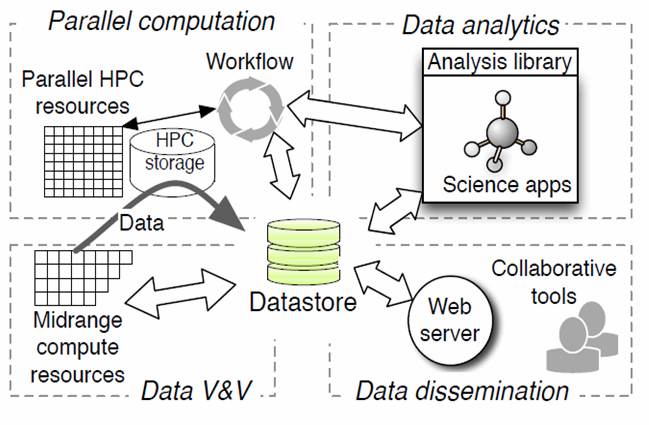
\includegraphics[height=1.3in,width=2.0in,viewport=0 0 680 460,clip]{Figures/Parallel_computation.png}
%\caption{\fontsize{5.2pt}{2.5pt}\selectfont{\textrm{High throughput architecture. The datastore serves all four functions, clockwise from upper-left:~Parallel computation, Data analytics, Data dissemination, and Data validation and verification. Ref\cite{unpublished}}}}%
%\label{parallel_computation}
%\end{figure} 
%}
%
\frame
{
	\frametitle{\textrm{VASP}计算的参数控制}
	\textcolor{red}{重点考虑}:~计算流程的脚本设计的任务之一,是设置\textrm{VASP~}的计算控制文件\textcolor{magenta}{\textrm{INCAR}}中的参数%(了解\textcolor{blue}{\textrm{INCAR}}文件)
	\begin{itemize}
		\item 计算量控制参数\\
			\textcolor{blue}{NKDIM~NBANDS~NEDOS~LDIM~LMDIM~NPLWV\\IRMAX~IRDMAX}
		\item 计算过程控制参数\\
			\textcolor{blue}{NWRITE~PREC~ISTART~ICHARG~ISPIN\\LNONCOLLINEAR~LSORBIT~INIWAV}
		\item 离子步计算控制参数\\
			\textcolor{blue}{EDIFFG~NSW~NBLOCK~\textcolor{red}{IBRION}~NFREE~ISIF~IWAVPR~LCORR}
		\item 电子步计算控制参数\\
			\textcolor{blue}{ENCUT~ENINI~ENAUG~NELM~EDIFF~NLSPLINE~LMAXPAQ~LMAXMIN~\textcolor{red}{IALGO}~LDIAG~LSUBROT~\textcolor{red}{IMIX}~\textcolor{red}{AMIX}~\textcolor{red}{AMIN}}
	\end{itemize}
}

\frame
{
	\frametitle{\textrm{VASP}计算的优化参数}
	\textcolor{red}{流程设计难点}:~围绕本课题复杂体系\textrm{VASP}的计算,通过脚本有效选取迭代、优化与收敛参数是难点\\
	\textrm{VASP}针对迭代、优化和收敛分别提供了优化算法\\
	(涵盖\textrm{SD}、\textrm{CG}、\textrm{RMM-DIIS}等):
	\begin{itemize}
		\item 原子受力和晶体结构优化(控制参数\textcolor{blue}{IBRION})
			\begin{itemize}
		        \setlength{\itemsep}{15pt}
		   \item \textrm{quasi-Newton~(RMM-DIIS)}:~\textcolor{blue}{IBRION}=1
		   \item \textrm{Conjugate-Gradient (CG)}:~\textcolor{blue}{IBRION}=2
		   \item \textrm{Damping factor($\alpha$=\textcolor{blue}{POTIM};~$\mu$=\textcolor{blue}{SMASS})}:~\textcolor{blue}{IBRION}=3
			\end{itemize}
	\end{itemize}
}

\frame
{
	\frametitle{\textrm{VASP}计算的优化参数}
	\begin{itemize}
		\item \textrm{Kohn-Sham~}方程迭代对角化与电子结构计算
			\begin{itemize}
		\item \textcolor{blue}{IALGO}=\textcolor{red}{\textrm{38}}:~\textrm{Davidson block iteration}
			\begin{description}
				\item[\textcolor{blue}{ALGO}] = \textrm{Normal}
			\end{description}
		\item \textcolor{blue}{IALGO}=\textcolor{red}{\textrm{48}}:~\textrm{Preconditioned residuum-minimization} 
			\begin{description}
				\item[\textcolor{blue}{ALGO}]=\textrm{Fast~{(RMM-DIIS)}}
			\end{description}
		\item \textcolor{blue}{IALGO}= \textrm{53}
			\begin{description}
				\item[\textcolor{blue}{ALGO}]=\textrm{Damped} 
			\end{description}
		\item \textcolor{blue}{IALGO}= \textrm{54}:~\textrm{damped MD}
		\item \textcolor{blue}{IALGO}= \textrm{58}:~\textrm{Preconditioned CG}
			\begin{description}
				\item[\textcolor{blue}{ALGO}]=\textrm{All} 
			\end{description}
		\item \textcolor{blue}{IALGO}= \textcolor{red}{\textrm{90}}:~\textrm{Exact Diagonalization}
	\end{itemize}
	\end{itemize}
}

\frame
{
	\frametitle{\textrm{VASP}计算的优化参数}
	\begin{itemize}
		\item 电荷密度混合与迭代收敛
			\begin{itemize} 
		   \item \fontsize{9.2pt}{1.9pt}{\selectfont\textrm{No mixing}}:~\textcolor{blue}{IMIX}=0~ $\rho_{\mathrm{mixed}}=\rho_{\mathrm{out}}$
		   \item \fontsize{9.2pt}{1.9pt}{\selectfont\textrm{Kerker mixing}}:~\textcolor{blue}{IMIX}=1\\
			   $\rho_{\mathrm{mixed}}(\vec G)=\rho_{\mathrm{in}}(\vec G)+\textcolor{blue}{\mathrm{AMIX}}\dfrac{\vec G^2}{\vec G^2+\textcolor{blue}{\mathrm{BMIX}}^2}(\rho_{\mathrm{out}}(\vec G)-\rho_{\mathrm{in}}(\vec G))$ 
		   \item \fontsize{9.2pt}{1.9pt}{\selectfont\textrm{Damping factor($\mu$=\textcolor{magenta}{AMIN})}}:~\textcolor{blue}{IMIX}=2\\
			   $\ddot{\rho}_{\mathrm{in}}(\vec G)=2\cdot\textcolor{blue}{\mathrm{AMIX}}\dfrac{\vec G^2}{\vec G^2+\textcolor{blue}{\mathrm{BMIX}}^2}(\rho_{\mathrm{out}}(\vec G)-\rho_{\mathrm{in}}(\vec G))-\mu\cdot\dot{\rho}(\vec G)$
			\begin{displaymath}
				\begin{aligned}
					\dot{\vec\rho}_{\mathrm{N+1/2}}&=\bigg((1-\mu/2)\dot{\vec\rho}_{\mathrm{N}-1/2}-2\cdot\vec F_{\mathrm{N}}\bigg)/(1+\mu/2)\\
					\vec F(\vec G)&=\textcolor{blue}{\mathrm{AMIX}}\dfrac{\vec G^2}{\vec G^2+\textcolor{blue}{\mathrm{BMIX}}^2}(\rho_{\mathrm{out}}(\vec G)-\rho_{\mathrm{in}}(\vec G))\\
					\dot{\vec\rho}_{\mathrm{N+1}}&=\dot{\vec\rho}_{\mathrm{N}}+\dot{\vec\rho}_{\mathrm{N}+1/2}
				\end{aligned}
			\end{displaymath}
		   \item \fontsize{9.2pt}{1.9pt}{\selectfont\textrm{Pulay' mixing or Broyden's method~(\textcolor{blue}{WC})}}:~\textcolor{blue}{IMIX}=4\\
			\end{itemize}
	\end{itemize}
}

\frame
{
	\frametitle{自动流程的设计与开发}
	\textcolor{red}{设计的目标}:~围绕\textrm{VASP~}作业并发提交与过程监控
		%\item 计算过程的控制方式
	\begin{itemize}
		\item \textcolor{purple}{\textrm{Atomate}}:~数据库支持的计算流程控制:~适合复杂的\textrm{~VASP~}计算
\begin{figure}[h!]
\centering
\vspace*{-0.1in}
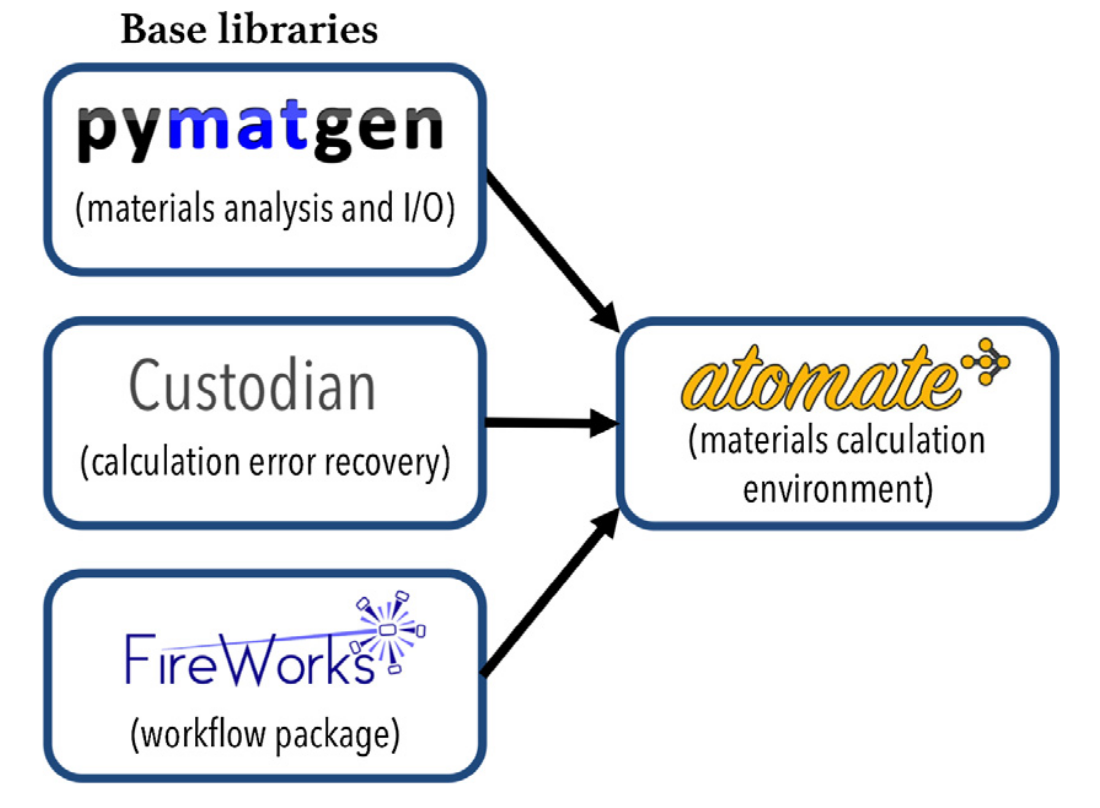
\includegraphics[height=0.8in,width=1.4in,viewport=0 0 820 630,clip]{Figures/Atomate_comp.png}
\hskip 15pt
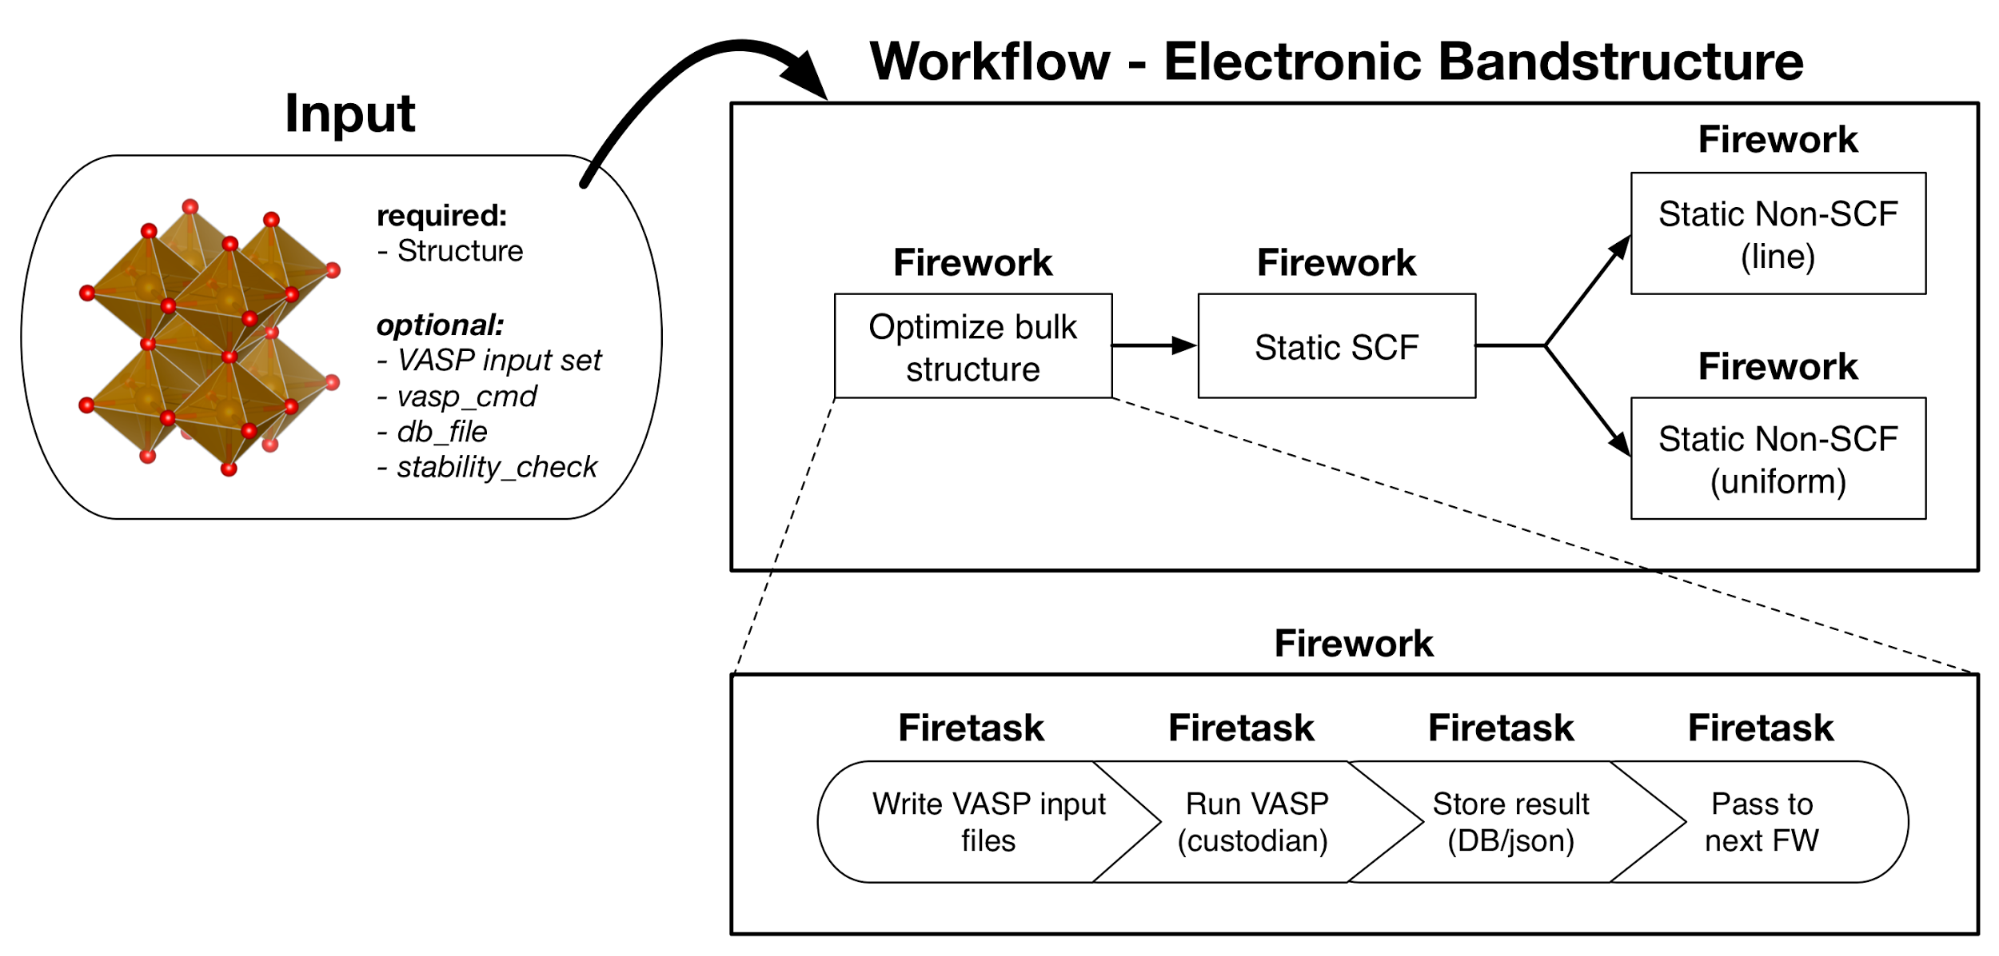
\includegraphics[height=0.8in]{Figures/bandstructure_wf.png}
%\caption{\fontsize{7.2pt}{4.2pt}\selectfont{\textrm{The integrated calculator in ASE (Atomic Simulation Environment).}}}%
\label{Logo_QM-MM}
\end{figure} 
		\item \textcolor{purple}{\textrm{ASE}}:~模块加载式计算流程控制:~简单灵活,支持软件多样性\\
\begin{figure}[h!]
\centering
\vspace*{-0.05in}
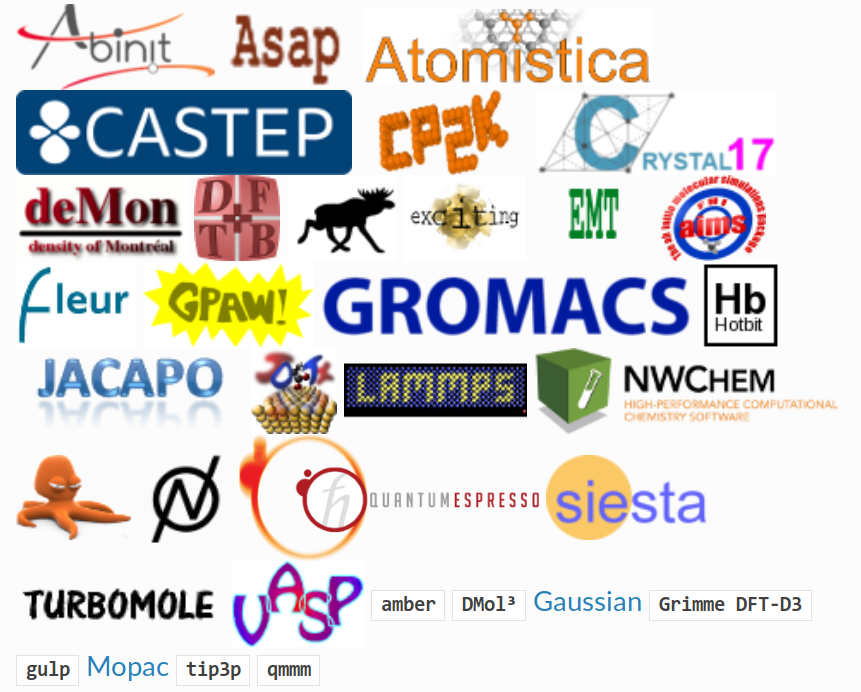
\includegraphics[height=1.0in,width=1.4in,viewport=0 0 638 530,clip]{Figures/ASE_calculator.png}
\label{bandstructure_wf}
\end{figure} 
%				\textcolor{red}{不足}:~流程设计与并发复杂度高
	\end{itemize}
}

%\frame
%{
%	\frametitle{国外已有的计算平台}
%\begin{figure}[h!]
%\centering
%\vspace{-15.5pt}
%\subfigure[\fontsize{7.5pt}{6.2pt}\selectfont{\textrm{Auto-FLOW (AFLOW)}\upcite{CMS58-227_2012}}]{
%\label{AFLOW_data_flow}
%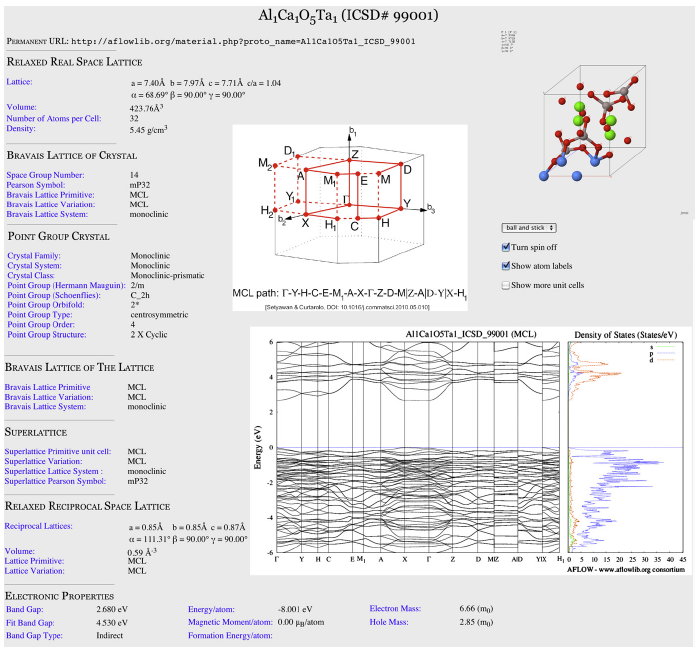
\includegraphics[height=1.2in,width=1.6in,viewport=0 0 720 660,clip]{Figures/AFLOW_database.png}}
%\subfigure[\fontsize{7.5pt}{6.2pt}\selectfont{\textrm{Material Project (MP)}\upcite{CMS97-209_2015}}]{
%\label{MP_commp_infrastructure}
%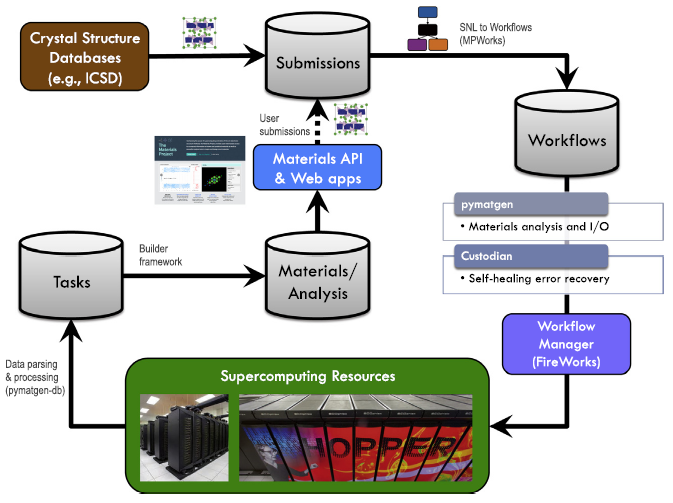
\includegraphics[height=1.2in,width=1.7in,viewport=0 0 670 530,clip]{Figures/MP_comp_infrastructure.png}}
%\subfigure[\fontsize{3.5pt}{3.2pt}\selectfont{\textrm{Quantum Materials Informatics Project (QMIP)}\upcite{url_QMIP}}]{
%\label{QMIP_Shame}
%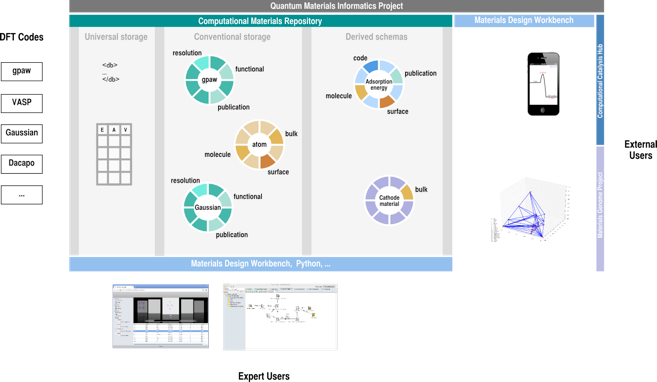
\includegraphics[height=1.2in,width=1.7in,viewport=0 0 670 420,clip]{Figures/QMIP_shame.png}}
%\subfigure[\fontsize{6.5pt}{5.2pt}\selectfont{\textrm{Clean Energy Project (CEP)}\upcite{JPCL2-2241_2011}}]{
%\label{CEP_structure_flow}
%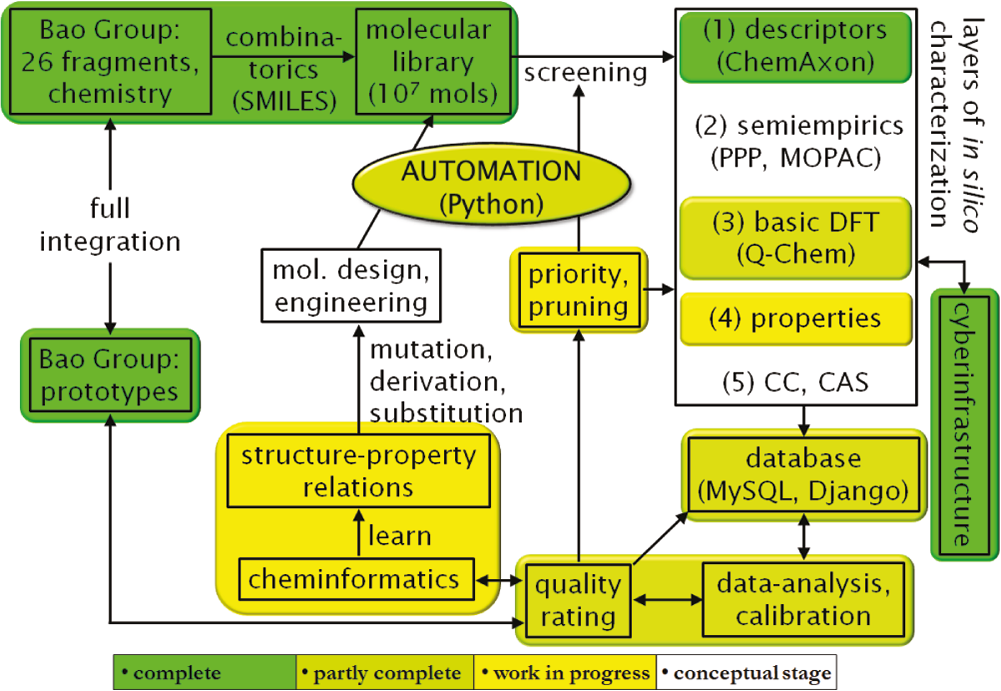
\includegraphics[height=1.2in,width=1.6in,viewport=0 0 1020 730,clip]{Figures/CEP_structure_flow.png}}
%%\caption{}%
%\label{Auto_Flow_Platform}
%\end{figure}
%}

%\frame
%{
%	\frametitle{\textrm{计算平台}}
%\begin{figure}[h!]
%\centering
%\vspace*{-0.2in}
%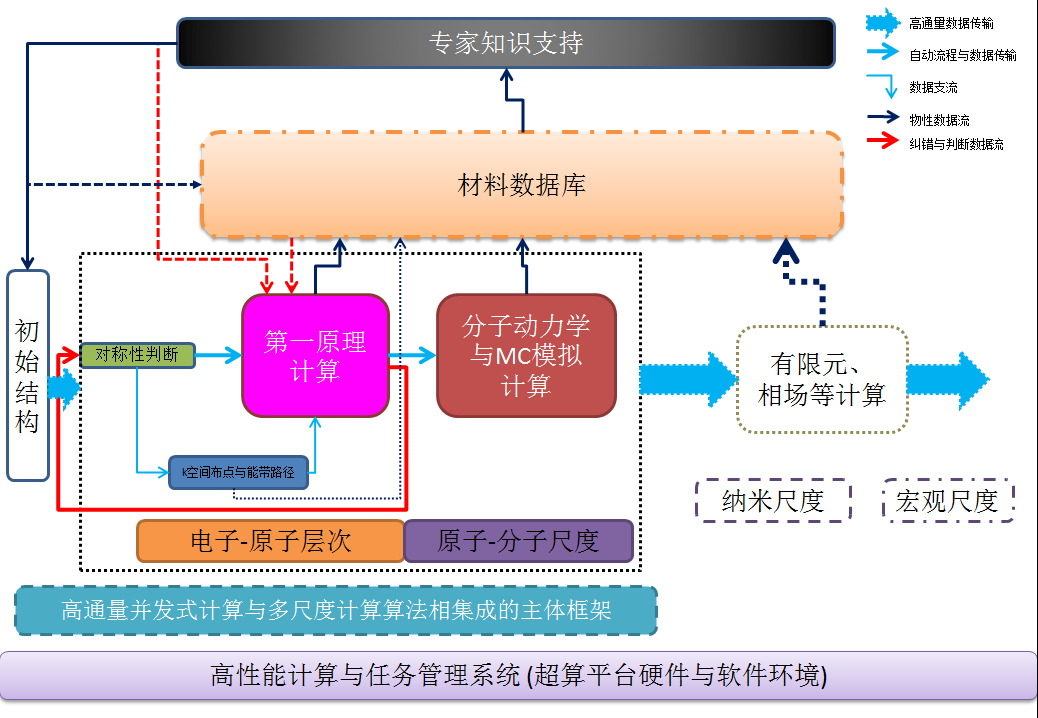
\includegraphics[height=2.6in,width=3.6in,viewport=0 0 1038 730,clip]{Figures/Auto_Flow.png}
%\caption{\fontsize{7.2pt}{4.2pt}\selectfont{\textrm{The schematic framework and platform of our project.}}}%
%\label{Auto_Flow}
%\end{figure} 
%}
%
%\frame
%{
%	\frametitle{\textrm{ASE}:~接口丰富的适应性计算平台}
%\begin{figure}[h!]
%\centering
%\vspace*{-0.2in}
%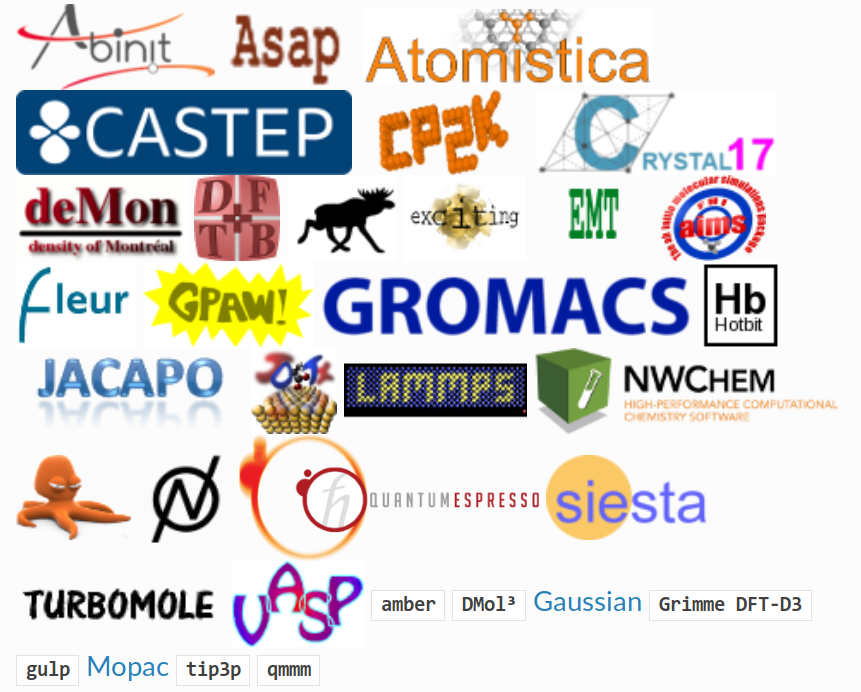
\includegraphics[height=2.1in,width=2.5in,viewport=0 0 638 530,clip]{Figures/ASE_calculator.png}
%\caption{\fontsize{7.2pt}{4.2pt}\selectfont{\textrm{The integrated calculator in ASE (Atomic Simulation Environment).}}}%
%\label{Logo_QM-MM}
%\end{figure} 
%}
%
%\frame
%{
%	\frametitle{\textrm{计算平台的作业自动提交:~基于\textrm{ASE}}}
%\begin{figure}[h!]
%\centering
%\vspace*{-0.2in}
%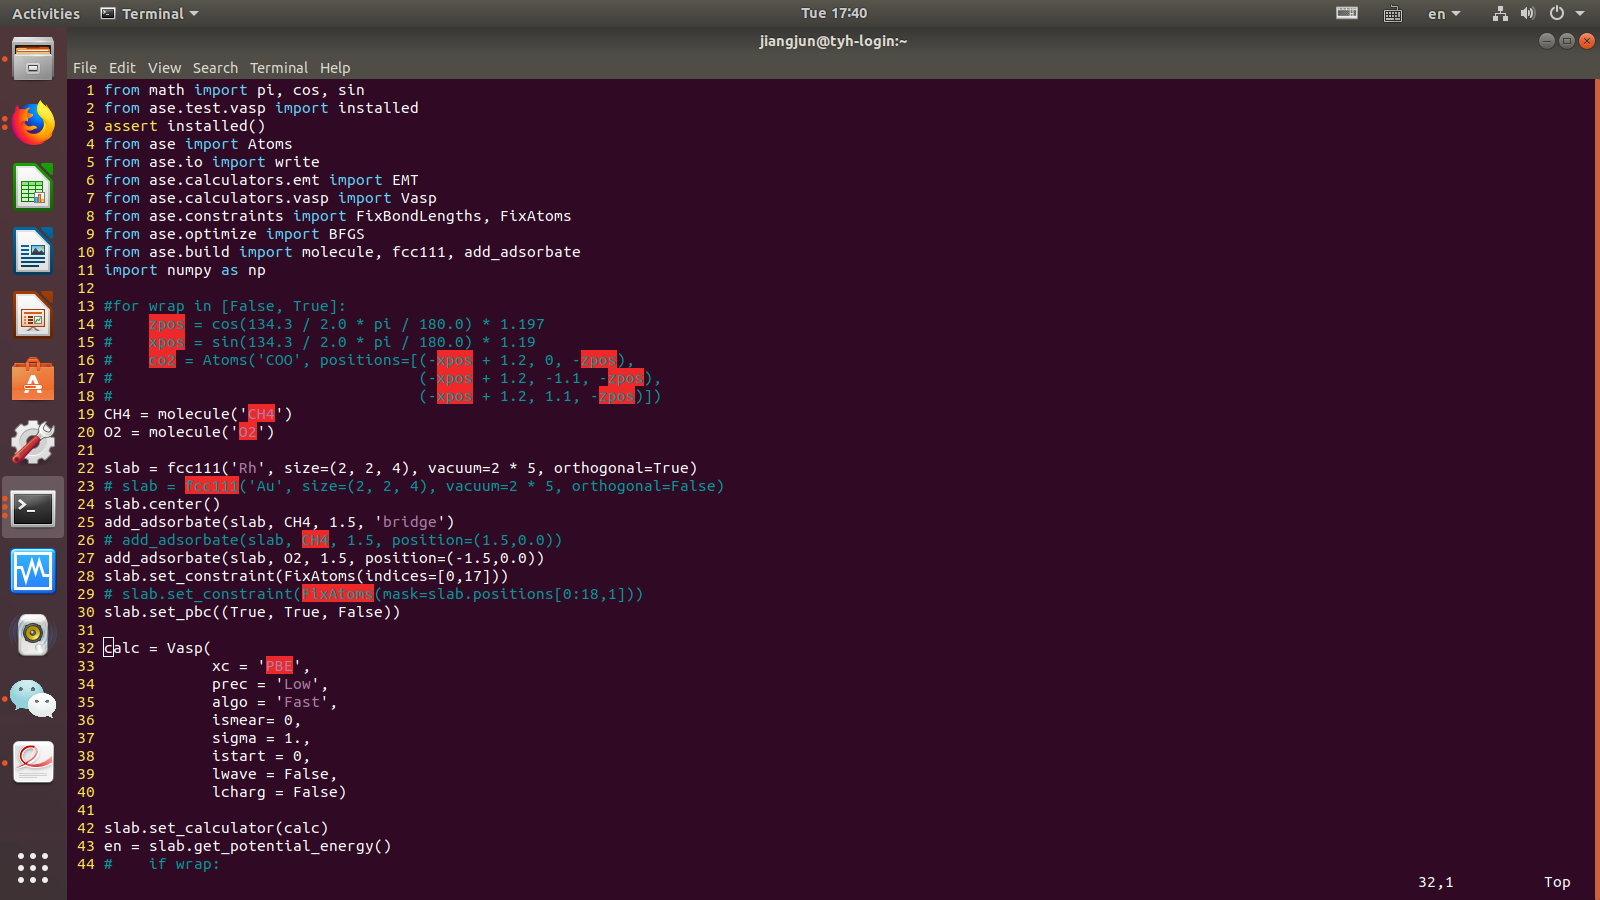
\includegraphics[height=3.1in,width=2.5in,viewport=75 0 725 820,clip]{Figures/ASE_app.png}
%%\caption{\fontsize{7.2pt}{4.2pt}\selectfont{\textrm{The integrated calculator in ASE (Atomic Simulation Environment).}}}%
%\label{ASE_app}
%\end{figure} 
%}
%
%\frame
%{
%	\frametitle{\textrm{计算平台的结果展示:~基于\textrm{MP}}}
%\begin{figure}[h!]
%\centering
%\vspace*{-0.2in}
%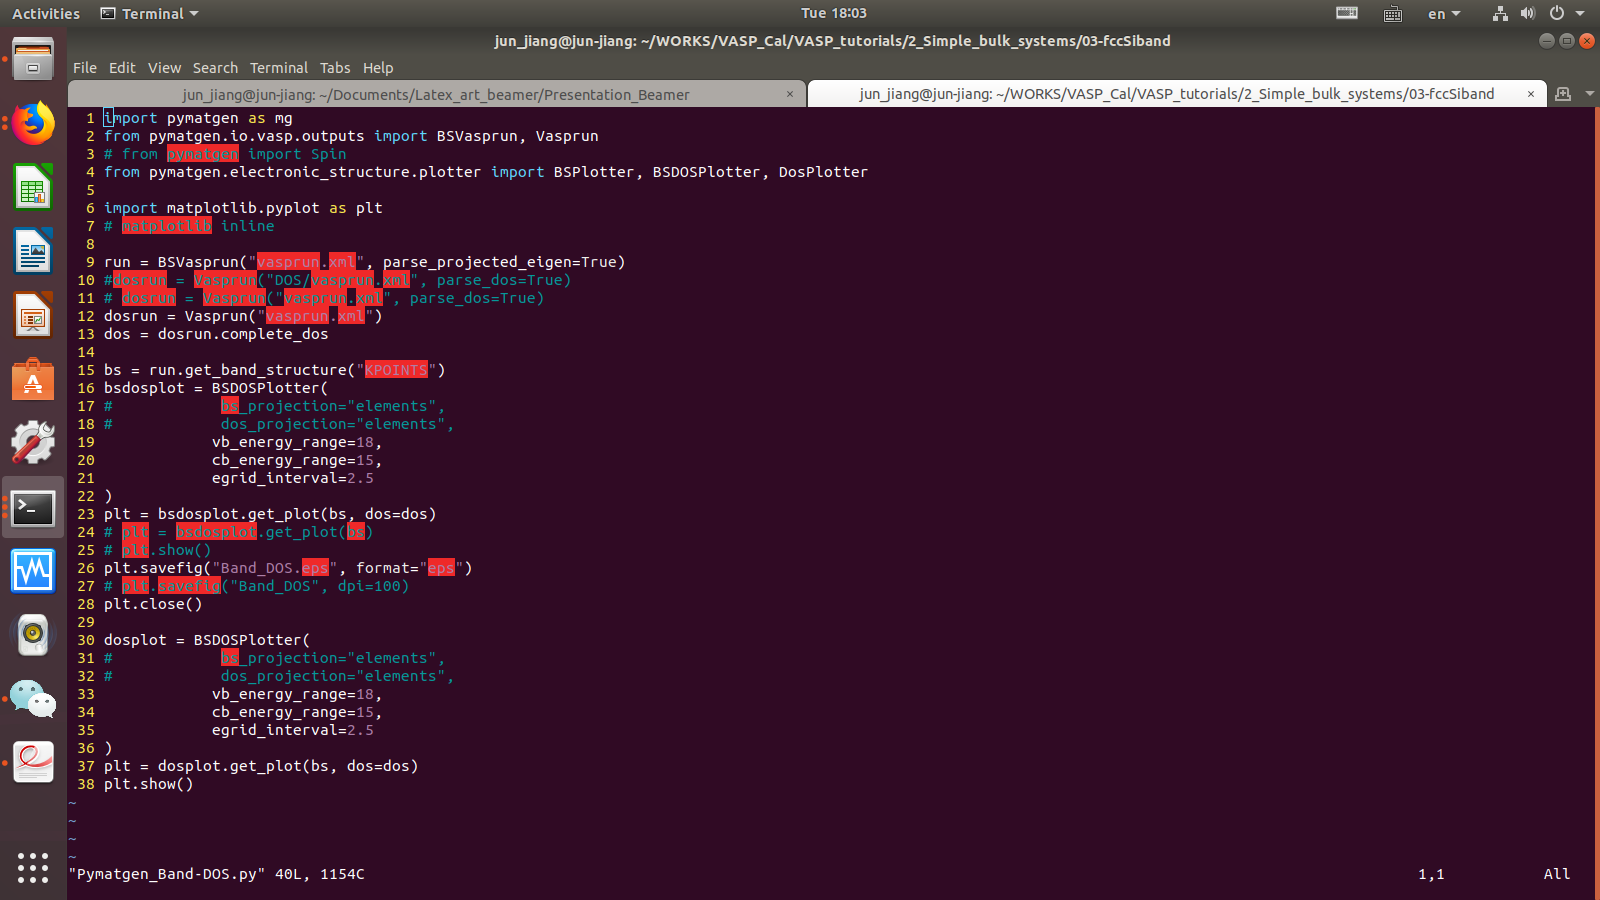
\includegraphics[height=3.1in,width=3.6in,viewport=73 80 880 790,clip]{Figures/Pymatgen_app.png}
%%\caption{\fontsize{7.2pt}{4.2pt}\selectfont{\textrm{The integrated calculator in ASE (Atomic Simulation Environment).}}}%
%\label{Pymatgen_app}
%\end{figure} 
%}
%
\frame
{
	\frametitle{自动流程软件的脚本设计}
%	\textcolor{purple}{\textrm{ASE~}}和\textcolor{brown}{\textrm{MP~}}(通过\textcolor{purple}{\textrm{Atomate}~}集成\textcolor{purple}{\textrm{Pymatgen}}、\textcolor{purple}{\textrm{FireWorks}}、\textcolor{purple}{\textrm{Custodian}})自动流程工作模式分析
	\textcolor{blue}{自动流程软件的脚本设计的技术路线}
	\begin{enumerate}
		\item \textcolor{purple}{\textrm{ASE~}}和\textcolor{purple}{\textrm{Atomate~}}整合成适应本课题计算的计算流程
		\item 通过增加计算流程中的脚本控制,优选合适的\textcolor{magenta}{\textrm{~INCAR}}~参数,满足复杂体系的计算需求
		\item 容错机制的充实与完善:%~目前只有\textcolor{purple}{\textrm{Custodian}}提供了简单容错策略
	 \begin{itemize}
		 \item 方案1:~基于\textcolor{purple}{\textrm{Custodian}}简单容错的充实与完善%(\textcolor{red}{理解\textcolor{purple}{\textrm{Custodian}}容错模式})
		 \item 方案2:~基于\textcolor{purple}{\textrm{ASE}}开发容错模块(脚本模式运行)
	 \end{itemize}
	\end{enumerate}
	\textcolor{blue}{自动流程软件的脚本设计的基本要求}
				\begin{itemize}
					\item 一定的\textrm{Python~}语言基础
					\item 对\textcolor{purple}{\textrm{ASE~}}和\textcolor{purple}{\textrm{Atomate~}}的功能模块有一定了解
				\end{itemize}
}

\frame
{
	\frametitle{\textrm{应用示例:~\textrm{MgO}}}
	算例来源:~\fontsize{7.5pt}{6.2pt}\selectfont{\url{https://atomate.org/running_workflows.html}}
\begin{figure}[h!]
\centering
\vspace*{-0.05in}
\hspace*{-0.10in}
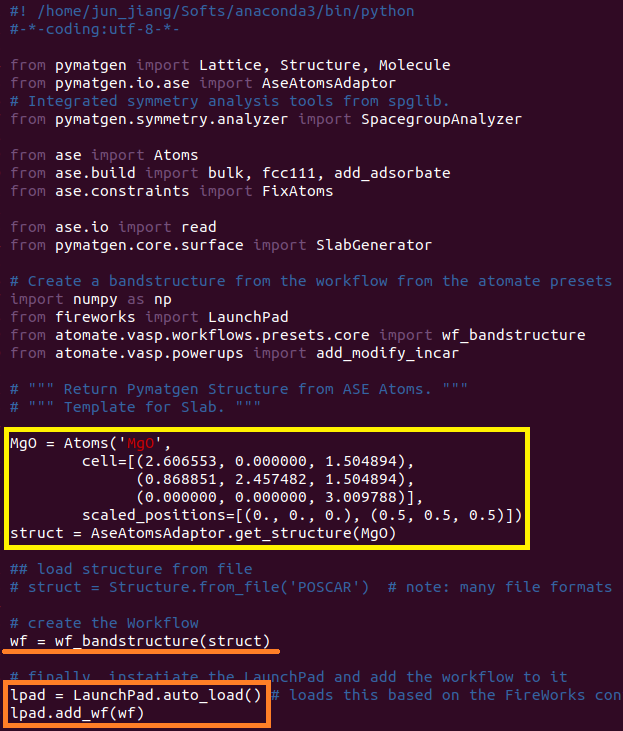
\includegraphics[height=2.6in,width=2.2in,viewport=0 0 475 515,clip]{Figures/Atomate-ASE_MgO.png}
%\caption{\fontsize{7.2pt}{4.2pt}\selectfont{\textrm{The integrated calculator in ASE (Atomic Simulation Environment).}}}%
\label{Atomate-ASE_MgO}
\end{figure} 
}

\frame
{
	\frametitle{应用示例:~\textrm{MgO~Band}}
\begin{figure}[h!]
\centering
\vspace*{-0.2in}
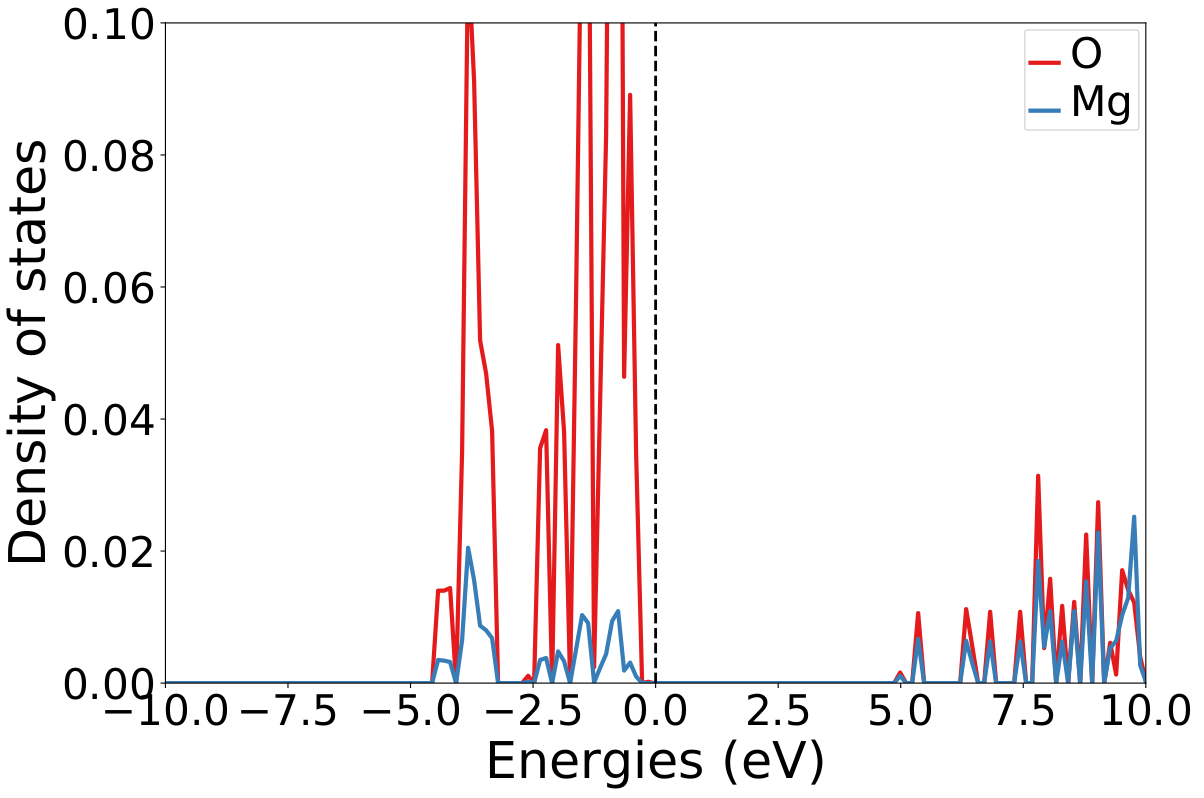
\includegraphics[height=1.5in,width=2.3in,viewport=0 0 900 600,clip]{Figures/Atomate_MgO-DOS.png}
\vskip 1pt
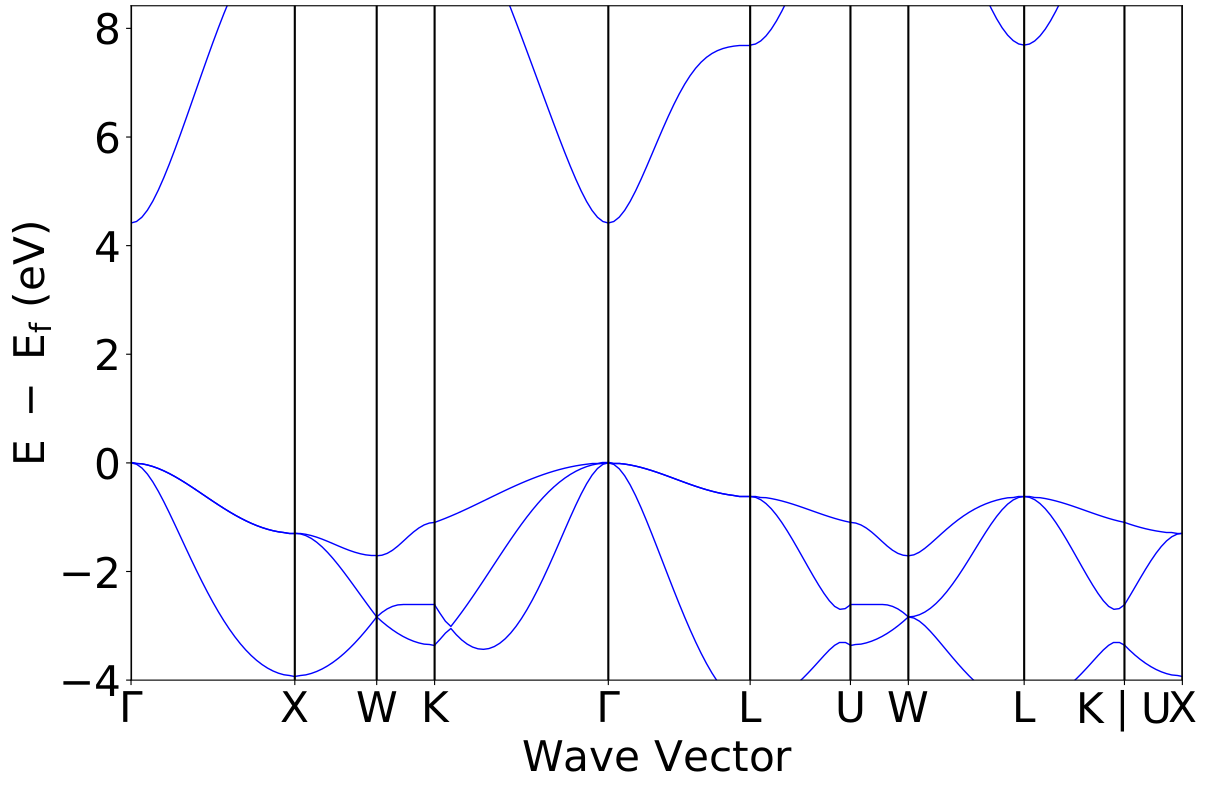
\includegraphics[height=1.5in,width=2.3in,viewport=0 0 900 600,clip]{Figures/Atomate_MgO-Band.png}
%\caption{\fontsize{7.2pt}{4.2pt}\selectfont{\textrm{The integrated calculator in Atomate-ASE.}}}%
\label{Atomate_MgO-DOS}
\end{figure} 
}


\section{空间群对称性分析模块与$\vec k$-\rm{path~}路径}
\frame
{
	\frametitle{传统能带计算的问题}
	初基原胞相同的材料电子结构表现出一定的相似性,但传统能带计算和表示的$\vec k$点路径($\vec k$-\textrm{Path})选择有着明显的人为性和任意性
%\vspace{10pt}
\begin{figure}[h!]
\centering
\hspace*{-0.30in}
\subfigure[\fontsize{6.5pt}{5.2pt}\selectfont{\textrm{Brillouin Zone of BCC lattice}}]{
\label{Brillouin_Zone_BCC}
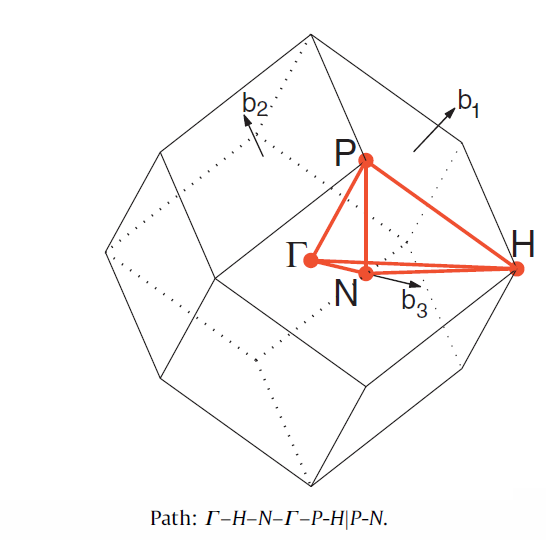
\includegraphics[height=1.5in,width=1.6in,viewport=00 0 550 520,clip]{Figures/Brillouin-Zone_BCC.png}}
%\vskip 0.10in
\subfigure[\textrm{Band structure of GeF$_4$}]{
\label{Band_Gap_GeF4}
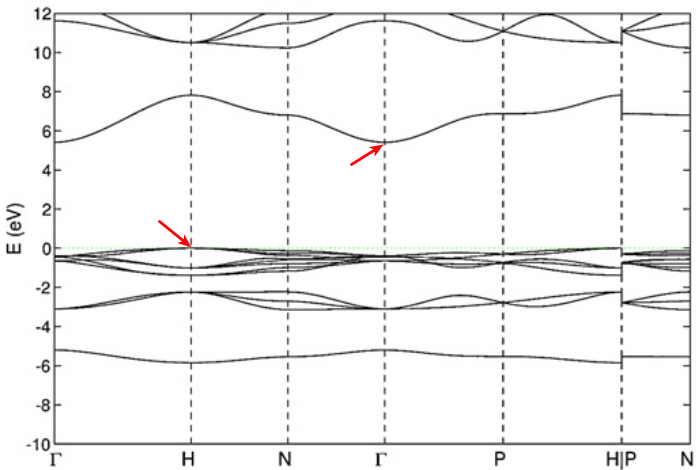
\includegraphics[height=1.05in,width=1.65in,viewport=0 0 750 500,clip]{Figures/Band-Struct_GeF4.png}}
\label{Band_Gap_BCC_GeF4}
\end{figure}
利用对称性模块实现\textcolor{red}{能带表示路径~$\vec k$-\textrm{path}“标准化”},对于高通量材料电子结构数据挖掘有着重要意义\upcite{CMS49-299_2010}
}

\frame
{
	\frametitle{对称性模块在计算流程中的作用与地位}
	对称性模块与材料物性计算
	\begin{itemize}
		\item \textcolor{blue}{第一原理计算中,材料初始结构经过弛豫会引起晶胞参数和原子坐标改变,体系对称性也可能发生变化。}
		\item \textcolor{blue}{材料的电子能带结构表示与所属空间群密切关联}
		\item \textcolor{blue}{材料的物理力学性质和受力分析都与体系的对称性有关,对于复杂合金材料,这个问题更为重要}\\
			对称性分析是材料的力学计算的基本步骤之一
	\end{itemize}
	\vskip 20pt
	高通量自动流程中的对称性模块
	\begin{itemize}
		\item \textcolor{blue}{高通量计算中,利用对称性可以有效地降低计算量且不损失计算精度}
		\item \textcolor{purple}{\textrm{Atomate}}中“结构弛豫-静态计算-能带表示”自动流程引入文献\cite{CMS49-299_2010}的对称性模块,实现能带表示路径$\vec k$-\textrm{path}“标准化”,\textcolor{red}{但没有完整的空间群信息}
	\end{itemize}
}

\frame
{
	\frametitle{\textrm{VASP~}现有的对称性判断}
\begin{figure}[h!]
\centering
\hspace*{-0.28in}
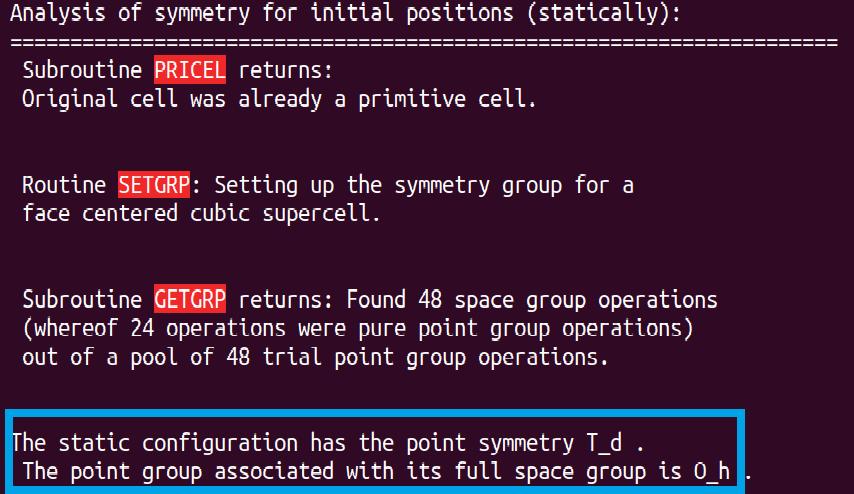
\includegraphics[height=2.0in,width=3.6in,viewport=0 0 600 380,clip]{Figures/VASP_Symmetry.png}
\caption{\textrm{Analysis of symmetry in VASP.}}
\label{VASP_symmetry}
\end{figure}
}

%\frame
%{
%	\frametitle{标准化的对称性模块}
%\begin{enumerate}
%   \setlength{\itemsep}{20pt}
%	\item 结构文件转换子模块:~\textcolor{magenta}{不同格式的结构文件间的相互转换}
%	\item 对称性分析功能子模块
%		\begin{itemize}
%			\item 确定原胞的点群、空间群和对称操作矩阵
%			\item 标准化的初基原胞(\textrm{primitive cell})
%				\vskip 2pt
%				\textcolor{magenta}{按晶轴长度和晶面夹角的大小确定晶格矢量排列顺序}
%		\end{itemize}
%	\item 标准化$\vec k$~点生成子模块\upcite{CMS49-299_2010}
%		\begin{itemize}
%			\item 确定14种\textrm{Bravais~}格子所有标准化\textrm{Wigner-Seitz~}原胞
%			\item 确定所有高对称性点的分数坐标和能带图中$\vec k$-\textrm{path}
%		\end{itemize}
%	\item 标准化结构参数的数据存储:~\textcolor{magenta}{元素、晶格、对称性等信息}
%\end{enumerate}
%}

%\frame
%{
%	\frametitle{标准化结构参数的数据存储子模块}
%\begin{figure}[h!]
%\centering
%\vspace*{-0.2in}
%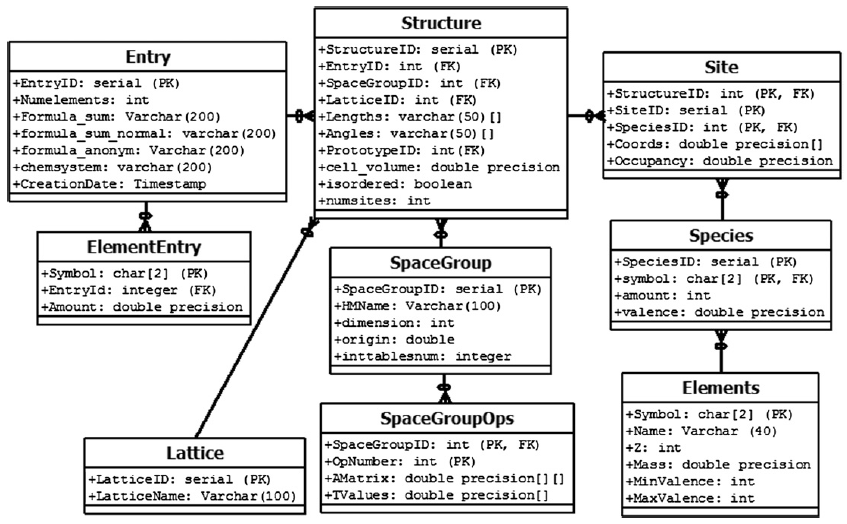
\includegraphics[height=2.5in,width=3.7in,viewport=0 0 850 540,clip]{Figures/MP_database_structure.png}
%\caption{\fontsize{7.2pt}{4.2pt}\selectfont{\textrm{Basic database schema for storing periodic crystal structures. Ref\cite{CMS50-2295_2011}}}}%
%\label{MP_structure_data}
%\end{figure} 
%}
%
\frame
{
	\frametitle{\textrm{VASP~}软件的对称性判断与功能解析}
	\textrm{VASP~}软件的对称性模块功能分析
	\begin{itemize}
		\item 模块\textcolor{blue}{\textbf{LATTYP}}:~晶胞结构的标准化
			\begin{enumerate}
				\item 根据\textcolor{blue}{\textrm{POSCAR}~}中的原始矢量,约化最小晶格矢量\\
				\item \textcolor{magenta}{晶格矢量标准化}:~按晶轴长度和晶面夹角的大小确定晶格矢量排列顺序
				\item 根据标准化的最小晶格矢量,确定晶体所属\textrm{Bravais~}格子和晶胞参数
			\end{enumerate}
		\item 模块\textcolor{blue}{\textbf{PRICEL}}:~确定初基原胞(\textrm{primitive cell})\\
			\begin{enumerate}
				\item 根据晶胞中原子类型与原子数目判断初基原胞数目
				\item 根据同类原子位置确定初基原胞矢量
				\item 初基原胞矢量标准化,判断\textrm{Bravais~}格子一致性
			\end{enumerate}
		\item \textcolor{magenta}{晶胞原子坐标标准化}:~原子坐标变换到$[-0.5,0.5)$
	\end{itemize}
		\textcolor{red}{晶胞原子坐标和初基原胞标准化是对称性分析的基础}
}

\frame
{
	\frametitle{\textrm{VASP~}点群对称性判断与晶胞选择}
	以面心立方的\textrm{Si~}为例,其结构和对应的\textrm{POSCAR~}文件可以选为
\begin{figure}[h!]
\centering
\vspace*{-0.1in}
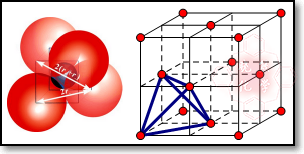
\includegraphics[height=1.5in,width=3.0in,viewport=0 0 350 160,clip]{Figures/FCC_Si.png}
\vskip 0.1in
\hspace*{-0.15in}
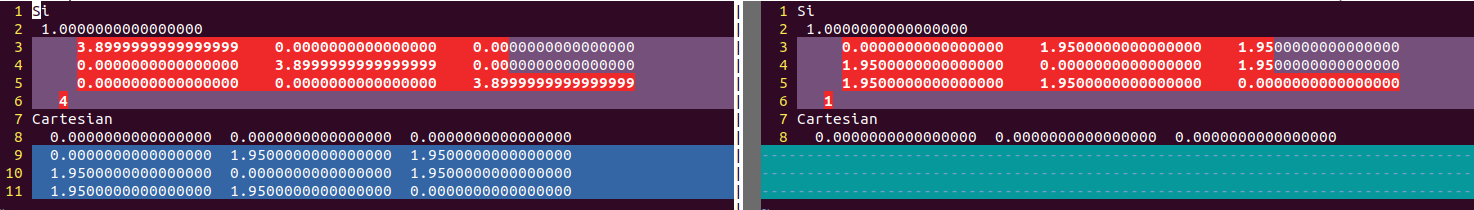
\includegraphics[height=0.7in,width=4.3in,viewport=0 0 1080 160,clip]{Figures/VASP_FCC_Si_POSCAR.png}
\caption{\fontsize{7.2pt}{4.2pt}\selectfont{\textrm{The FCC Si and its possible POSCAR for VASP.}}}%
\label{FCC_Si-POSCAR}
\end{figure} 
}

\frame
{
	\frametitle{\textrm{VASP~}点群对称性判断与晶胞选择}
	在\textrm{VASP~}中,对应的对称性判断为
\begin{figure}[h!]
\centering
\vspace*{-0.1in}
\hspace*{-0.15in}
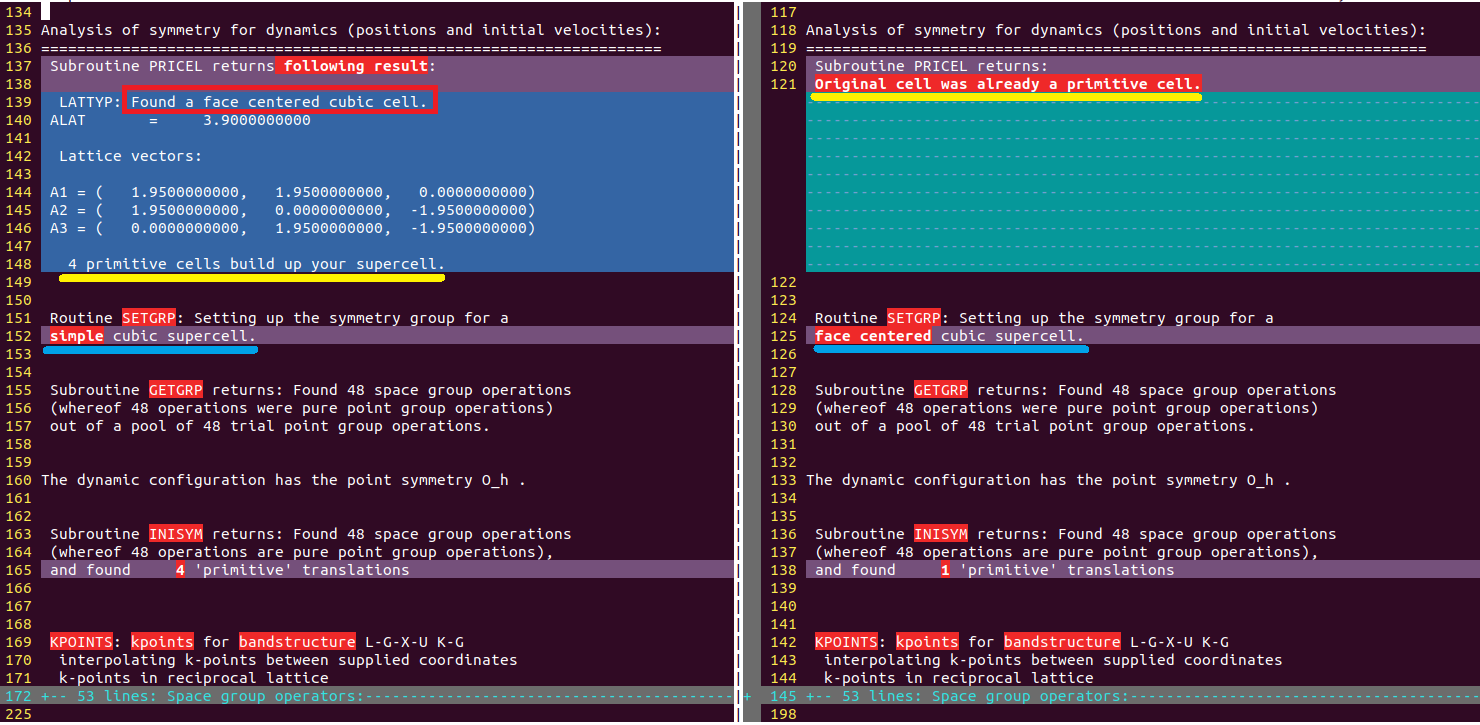
\includegraphics[height=2.3in,width=4.3in,viewport=0 0 1080 530,clip]{Figures/VASP_FCC_Si_symmetry.png}
%\caption{\fontsize{7.2pt}{4.2pt}\selectfont{\textrm{Basic database schema for storing periodic crystal structures. Ref\cite{CMS50-2295_2011}}}}%
\label{FCC_Si-OUTCAR}
\end{figure} 
}

\frame
{
	\frametitle{\textrm{VASP~}软件的对称性判断与功能解析}
	\textrm{VASP~}软件的\textcolor{red}{体系点群对称性确定}
	\begin{itemize}
		\item 模块\textcolor{blue}{\textbf{SETGRP}}:~确定晶体可能对应的标准点群
			\begin{enumerate}
				\item 根据\textrm{Bravais~}格子类型,确定许可点群的基本生成元素
				\item 根据点群基本生成元素,得到32点群全部对称操作矩阵
			\end{enumerate}
		\item 模块\textcolor{blue}{\textbf{GETGRP}}:~检查符合晶胞中原子位置的点群操作元素
			\begin{enumerate}
				\item 将晶胞所属\textrm{Bravais~}格子许可的点群依次作用于晶胞中的原子坐标
				\item 模块\textcolor{blue}{\textbf{CHKSYM}}:~检查对称操作元素能否将晶胞原子复原
			\begin{itemize}
				\item 所有的原子位置可重合~(纯粹的点群操作)
				\item 点群对称操作,须外加滑移对称性~(空间群操作)
				\item 原子位置无法重合~(不允许的对称操作)
			\end{itemize}
			\end{enumerate}
		\item 模块\textcolor{blue}{\textbf{PGROUP}}:~确定晶体实际所属点群
			\begin{enumerate}
				\item 根据原子坐标确定的对称操作数目和对称操作矩阵特征,确定晶胞所属点群
				\item 再次检查确定的点群操作元素能否使晶胞全部原子复原
			\end{enumerate}
	\end{itemize}
}

%\frame
%{
%	\frametitle{\textrm{VASP~}软件的对称性判断与能带绘制}
%	根据\textrm{VASP~}计算得到\textrm{FCC-Si}的电子结构:\textrm{DOS}
%\begin{figure}[h!]
%\centering
%\vspace*{-0.1in}
%\hspace*{-0.20in}
%\includegraphics[height=1.5in,width=2.2in,viewport=0 0 890 570,clip]{Figures/VASP_FCC_Si-DOS_4.eps}
%\hspace*{0.01in}
%\includegraphics[height=1.5in,width=2.2in,viewport=0 0 890 570,clip]{Figures/VASP_FCC_Si-DOS_1.eps}
%\caption{\fontsize{7.2pt}{4.2pt}\selectfont{\textrm{The Density of States of FCC-Si from VASP.}}}%
%\label{FCC_Si-DOS}
%\end{figure} 
%\vspace*{-0.2in}
%		\textcolor{blue}{初基原胞(\textrm{primitive cell})用能带表示电子结构:~包含对称性信息}\\
%\vspace*{0.1in}
%		\textcolor{red}{超晶胞(\textrm{super cell})适合用态密度表示电子结构信息}
%}
%

\frame
{
	\frametitle{对称性分析:~空间群对称性}
\begin{minipage}[b]{0.52\linewidth}
	空间群判断模块\textcolor{blue}{\textbf{SGROUP}}:~确定体系所属空间群
	\begin{enumerate}
		\item 通过检查晶胞中许可的平移操作数目,确定最终的点群和空间群的对应关系\\
			{\fontsize{7.2pt}{4.2pt}\selectfont{(32点群-230空间群对应列表)}}
		\item 根据确定的空间群名,输出对应的空间群操作表示矩阵\\{\fontsize{7.2pt}{4.2pt}\selectfont{(点群矩阵+平移矢量)}}
	\end{enumerate}
\end{minipage}
\hfill
\begin{minipage}[b]{0.46\linewidth}
\begin{figure}[h!]
\centering
\vspace*{-0.2in}
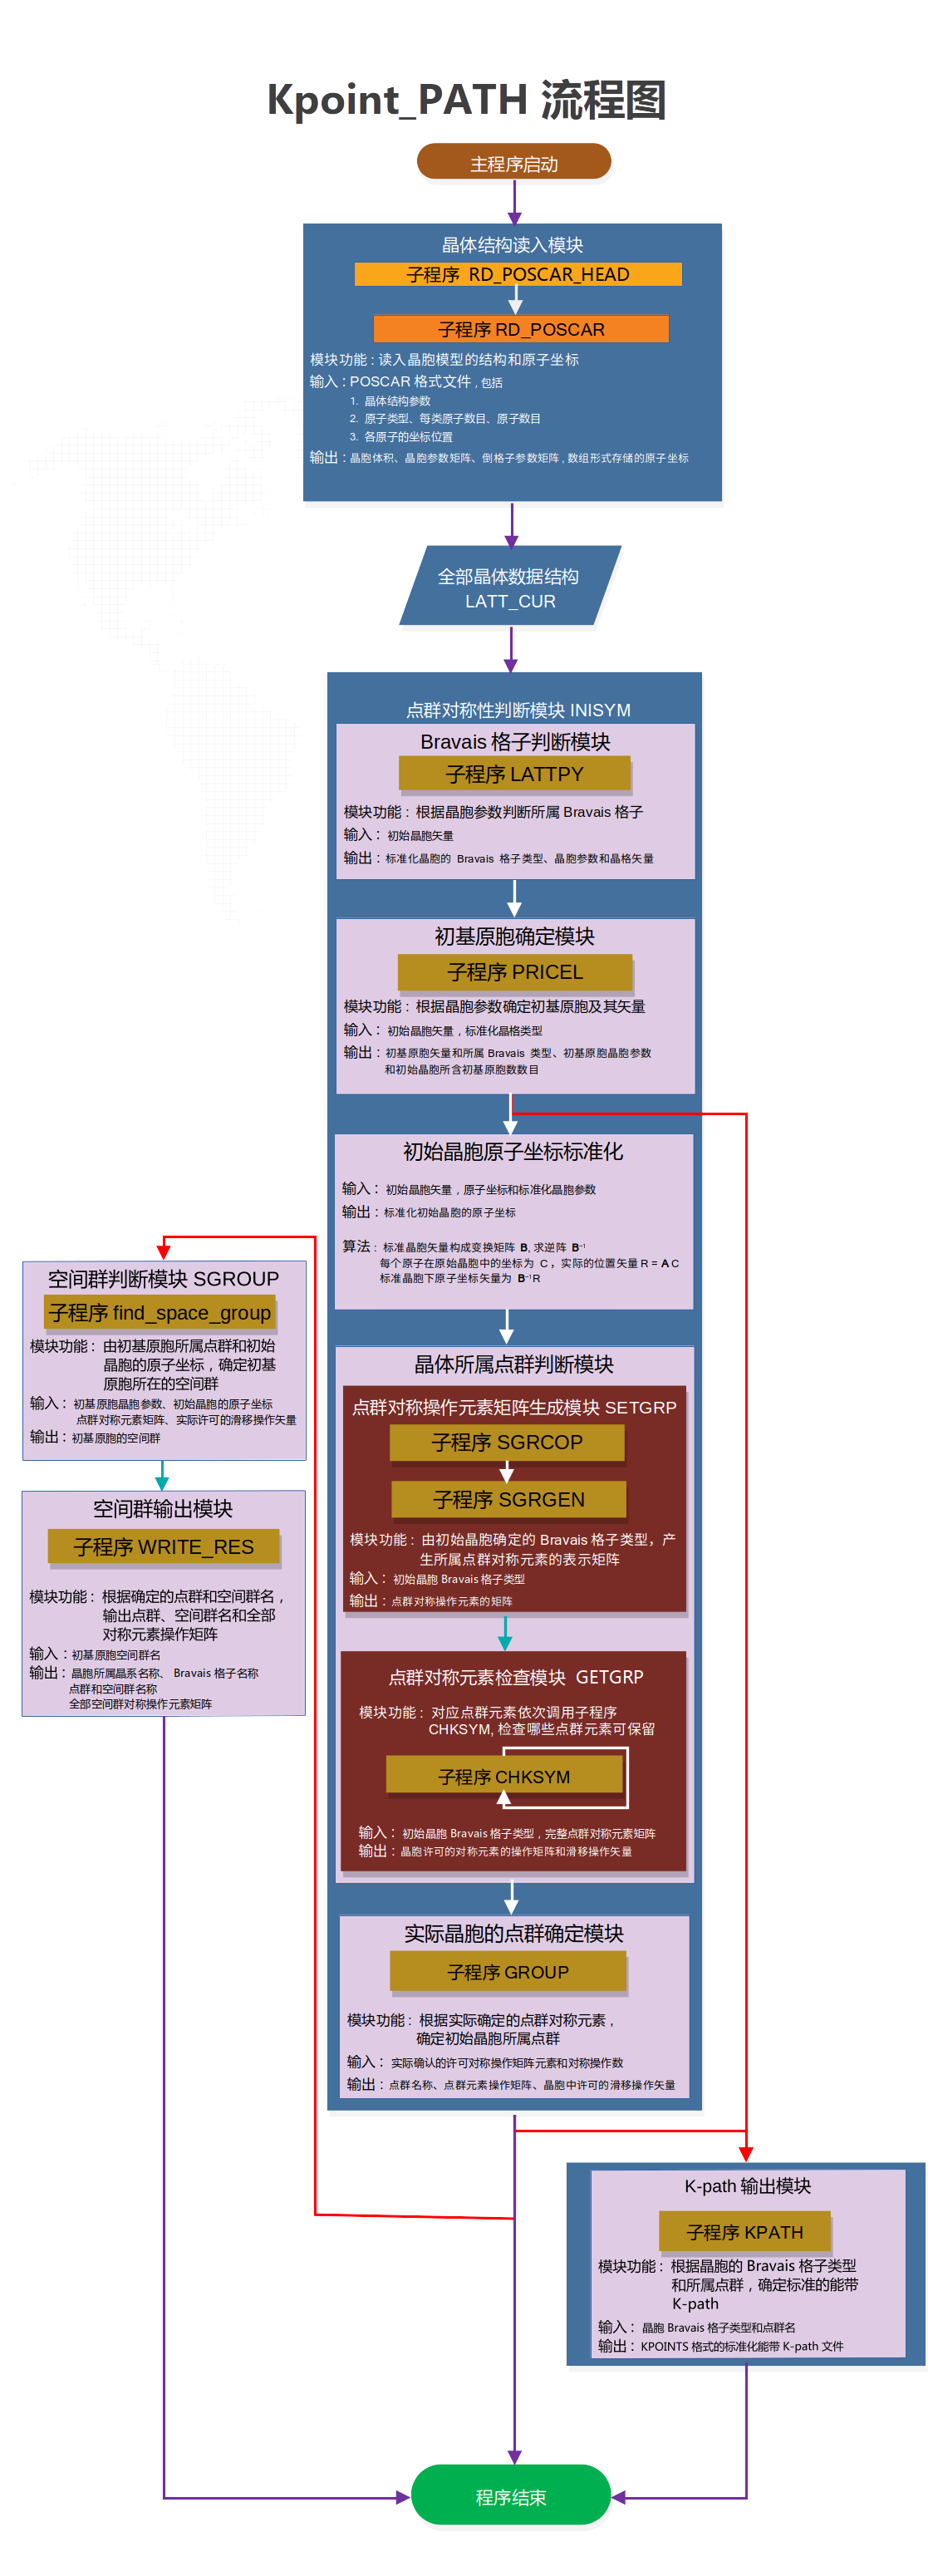
\includegraphics[height=3.05in,width=1.55in,viewport=0 50 840 2255,clip]{Figures/VASP_sym-detail.png}
\label{Space_Symmetry}
\end{figure} 
\end{minipage}
}

\frame
{
	\frametitle{对称性分析:~空间群对称性算例}
	基于\textrm{VASP~}代码开发的空间群分析:~\textrm{HCP-Si}结构对称性分析
\begin{figure}[h!]
\centering
%\vspace*{-0.1in}
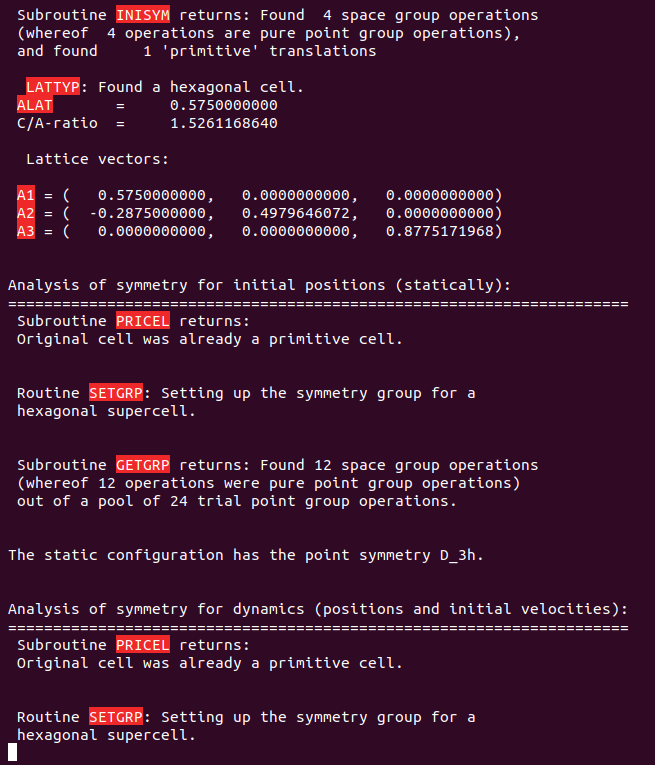
\includegraphics[height=2.2in,width=1.9in,viewport=0 0 520 570,clip]{Figures/HCP_Si_Symm-1.png}
\hspace*{0.01in}
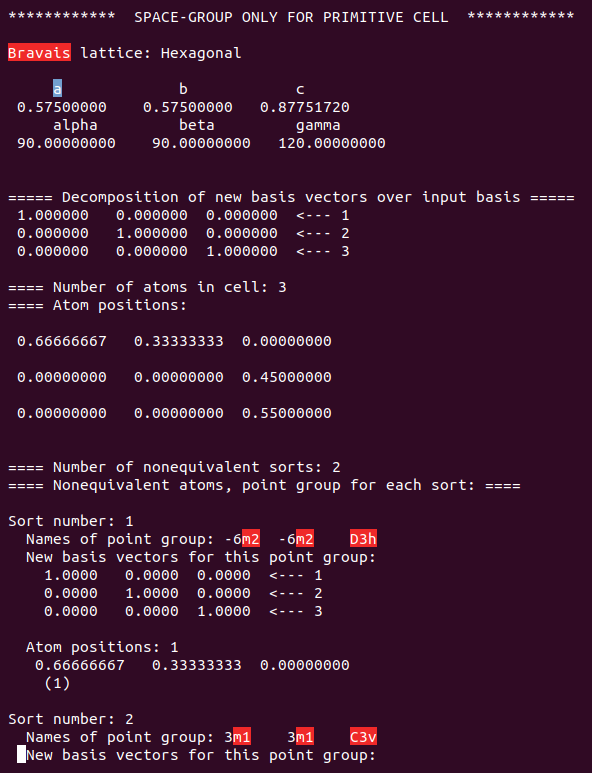
\includegraphics[height=2.2in,width=1.9in,viewport=0 0 520 580,clip]{Figures/HCP_Si_Symm-2.png}
\caption{\fontsize{7.2pt}{4.2pt}\selectfont{\textrm{Space-Group-Analysis of HCP-Si developed from VASP codes.}}}
\label{Symmetry_Analysis}
\end{figure} 
}

\frame
{
	\frametitle{对称性分析:~空间群对称性算例}
	基于\textrm{VASP~}代码开发的空间群分析:~\textrm{HCP-Si}结构对称性分析
\begin{figure}[h!]
\centering
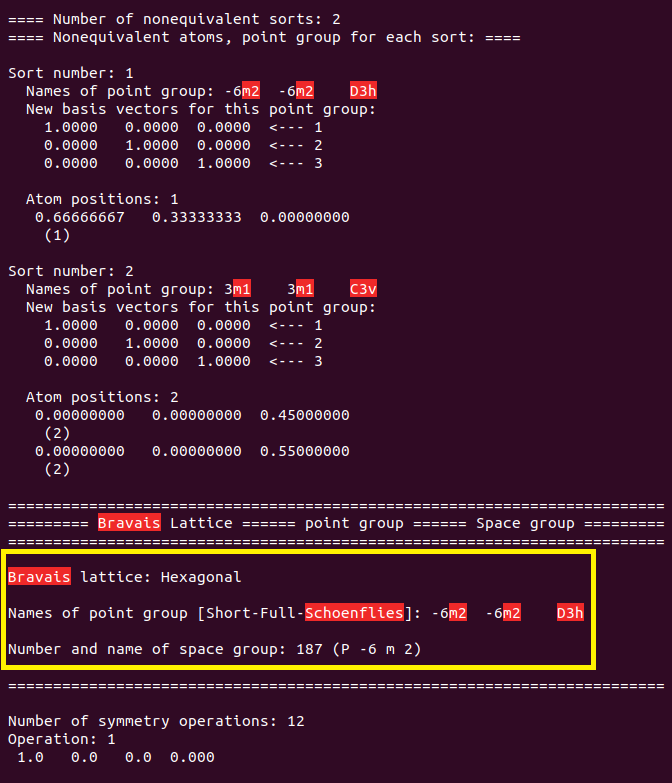
\includegraphics[height=2.3in,width=1.9in,viewport=0 0 520 600,clip]{Figures/HCP_Si_Symm-3.png}
\hspace*{0.01in}
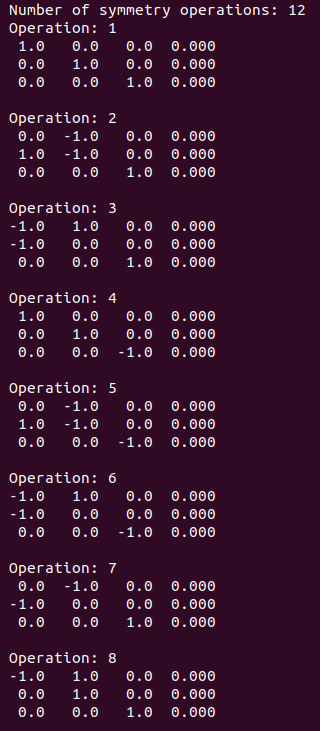
\includegraphics[height=2.3in,width=1.1in,viewport=0 0 270 560,clip]{Figures/HCP_Si_Symm-4.png}
\caption{\fontsize{7.2pt}{4.2pt}\selectfont{\textrm{Space-Group and the operating-matrix of HCP-Si.}}}
\label{Space_Group_Analysis}
\end{figure} 
}

%\frame
%{
%	\frametitle{对称性判断与能带路径标准化}
%	\begin{itemize}
%		\item 基于\textrm{VASP~}的对称性分析,标准化$\vec k$\textrm{-path~}路径的自动生成\\(\textcolor{purple}{针对不同\textrm{Bravais~}格子,枚举“标准化”路径的$\vec k$-点分布})
%	\end{itemize}
%\begin{figure}[h!]
%\centering
%\hspace*{-0.18in}
%\subfigure[{\fontsize{6.2pt}{4.2pt}\selectfont{\textrm{Procedure for Point-Group}}}]{
%\label{Procedure_Symmetry}
%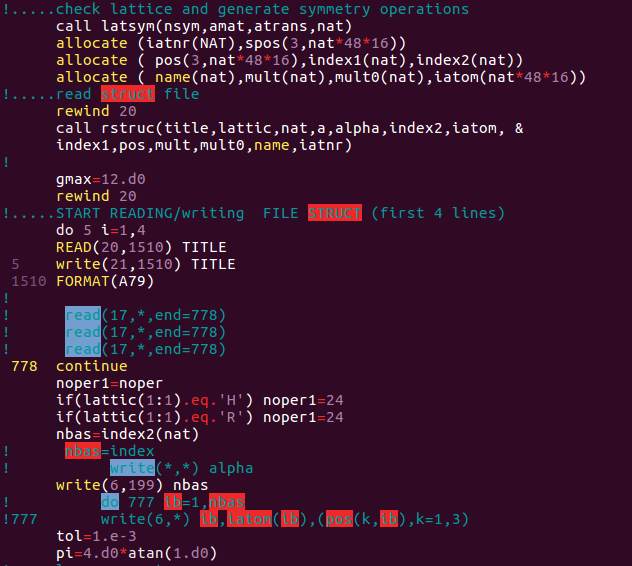
\includegraphics[height=2.0in,width=1.85in,viewport=0 0 580 570,clip]{Figures/Procedure_symmetry.png}}
%%\vskip 0.10in
%\subfigure[{\fontsize{6.2pt}{4.2pt}\selectfont{\textrm{Procedure for $\vec k$-path generation}}}]{
%\label{Procedure_sgroup}
%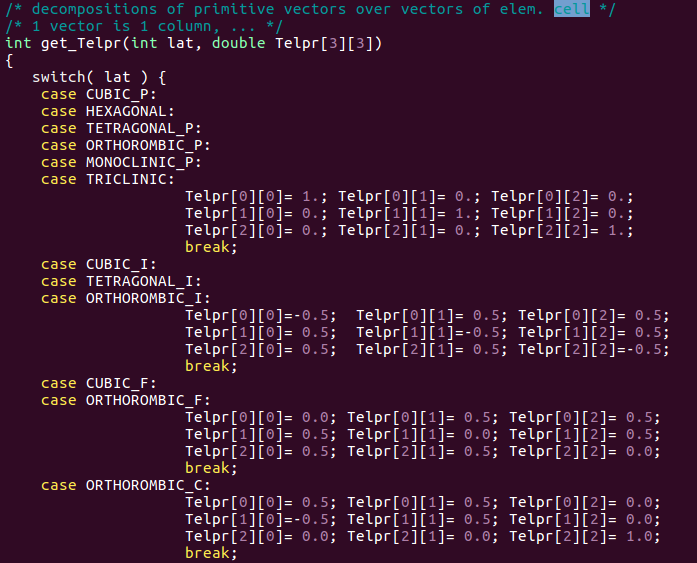
\includegraphics[height=2.0in,width=2.15in,viewport=0 0 670 570,clip]{Figures/Procedure_sgroup.png}}
%\label{Procedure_Symmetry_Sgroup}
%\end{figure}
%}
%
\frame
{
	\frametitle{对称性判断与能带路径标准化}
%	\frametitle{\textrm{VASP~}软件的对称性判断与能带$\vec k$-\textrm{path}}
	应用标准化能带$k$-\textrm{path}计算得到\textrm{FCC-Si}的\textrm{Band}\\{\fontsize{7.3pt}{6.2pt}\selectfont{(算例来源:~\url{http://cms.mpi.univie.ac.at/wiki/index.php/Fcc_Si_bandstructure})}}\\

\begin{figure}[h!]
\centering
\vspace*{-0.1in}
\includegraphics[height=2.0in,width=2.7in,viewport=0 0 890 570,clip]{Figures/FCC_Si-Band_pymatgen.eps}
\hspace*{0.01in}
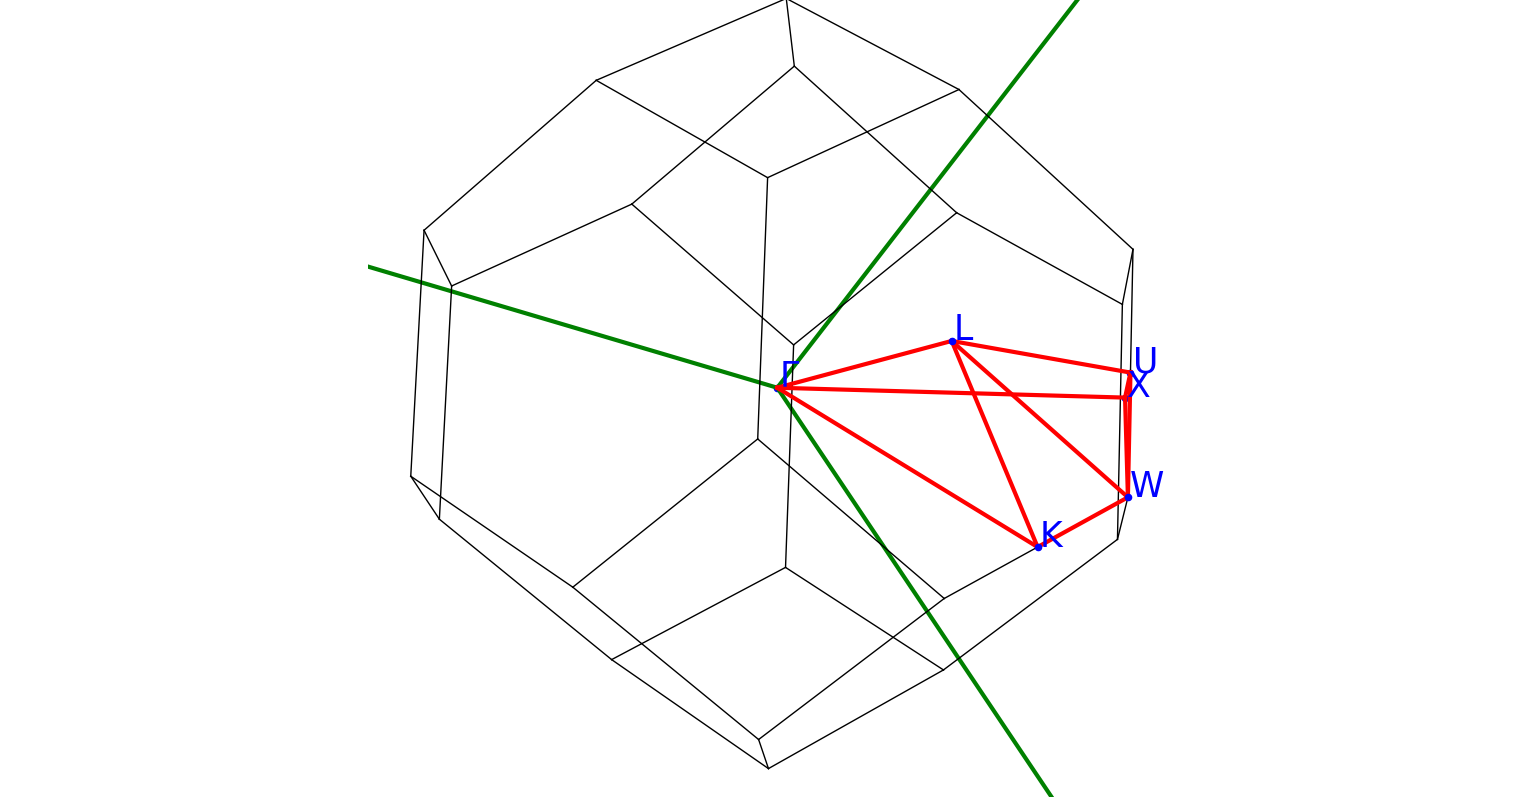
\includegraphics[height=1.5in,width=1.4in,viewport=280 0 850 600,clip]{Figures/FCC_Si-Brillouin-zone.png}
\caption{\fontsize{7.2pt}{4.2pt}\selectfont{\textrm{The Band-structure of FCC-Si and its standard $\vec k$-path.}}}%
\label{FCC_Si-Band}
\end{figure} 
}

\frame
{
	\frametitle{后续工作:~复杂体系的对称性}
	在\textrm{VASP~}中,$\mathrm{Ni}:\mathrm{Ni}_3\mathrm{Al}$体系的对称性判断,
\begin{figure}[h!]
\centering
%\vspace*{-0.1in}
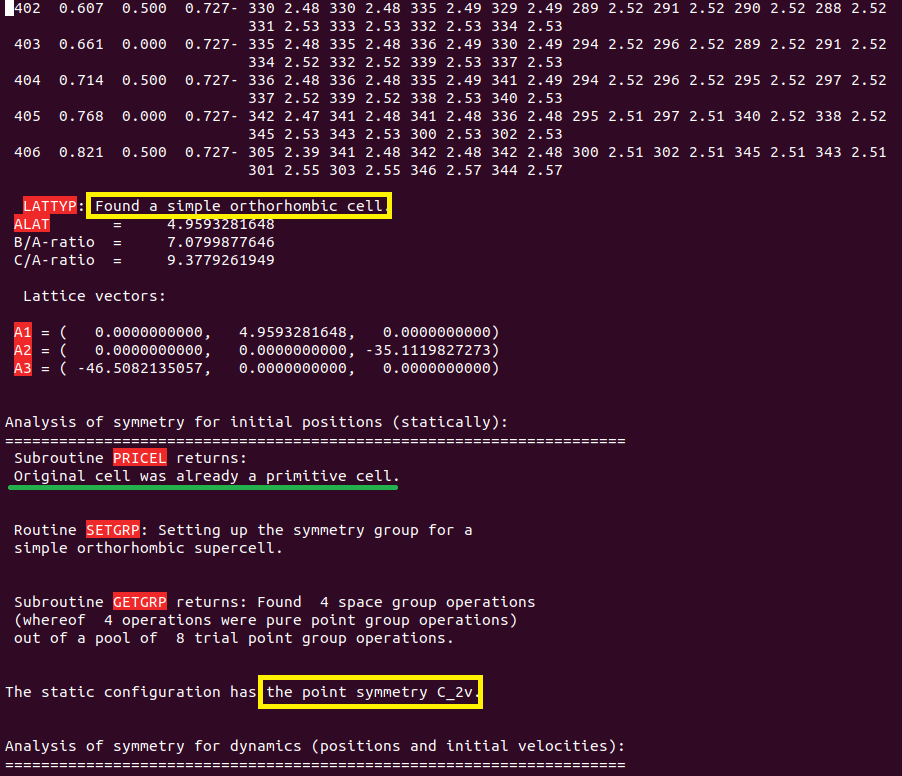
\includegraphics[height=2.6in,width=3.5in,viewport=0 0 680 530,clip]{Figures/VASP_Alloy_Ni-Al_symmetry.png}
%\caption{\fontsize{7.2pt}{4.2pt}\selectfont{\textrm{Basic database schema for storing periodic crystal structures. Ref\cite{CMS50-2295_2011}}}}%
\label{Alloy_Ni-Al-OUTCAR}
\end{figure} 
}

\frame
{
	\frametitle{后续工作:~复杂体系的对称性}
	\begin{itemize}
   		\setlength{\itemsep}{15pt}
		\item 当前各类软件的对称性判断模块都是在传统的群表示理论基础上开发的,主要适用于理想单晶的对称性判断
		\item 群论基本思想:~利用空间对称元素(平移或滑移、旋转、镜面、反演)约化重复单元中原子间的位置关系,实现对称问题的完备表示\\
			\textcolor{blue}{\textcolor{magenta}{初基原胞(\textrm{primitive cell})}是对称性判断的核心}
%		\item 程序中已经考虑了体系中平移操作的判断,但没有给出确定空间群(\textrm{Space-Group})方案
		\item 针对超晶胞(\textrm{super-cell}),特别是合金体系,\textcolor{red}{有更复杂的需求}
			\begin{itemize}
   				\setlength{\itemsep}{10pt}
				\item \underline{\textcolor{blue}{如何快速地确定\textcolor{magenta}{实际最小重复单元}及其元素组成}}
				\item \textcolor{blue}{\textcolor{magenta}{合金元素的存在}对于对称性判断的影响}
				\item \textcolor{blue}{\textcolor{magenta}{界面}与\textcolor{magenta}{多相合金}对于对称性判断的影响}
			\end{itemize}
	\end{itemize}
}

\section{\rm{VASP}的基态总能量计算与势能零点}
\frame
{
	\frametitle{晶体总能量的一般表示}
基于\textrm{DFT}的晶体总能量$E_T$由晶格中的电子能量$E_{e-e}$与离子实排斥能$E_{N-N}$之和:~
	\begin{displaymath}
		E_T=E_{e-e}+E_{N-N}=T[\rho]+E_{ext}+E_{\mathrm{Coul}}+E_{\mathrm{XC}}+E_{N-N}
	\end{displaymath}
根据\textrm{Kohn-Sham}方程,其中动能泛函用单电子能量表示为
\begin{displaymath}
	T[{\rho}]=\sum_in_i\langle\psi_i|\varepsilon_i-V_{\mathrm{KS}}|\psi_i\rangle
\end{displaymath}
$n_i$是$\psi_i$上的电子占据数,$\varepsilon_i$是其能量本征值,因此有
\begin{displaymath}
	\hspace*{-12.0pt}	E_T=\sum_in_i\varepsilon_i-\dfrac12\int\int\mathrm{d}\vec r\mathrm{d}\vec r\dfrac{\rho(\vec r)\rho(\vec r^{\prime})}{|\vec r-\vec r^{\prime}|}+\int\mathrm{d}\vec r\rho(\vec r)[\epsilon_{\mathrm{XC}}(\vec r)-V_{\mathrm{XC}}(\vec r)]+E_{N-N}
\end{displaymath}
}

\frame
{
	\frametitle{晶体总能量倒空间的表示}
周期体系的总能量表达式在动量空间($\vec K$空间)计算更方便
\begin{displaymath}
	\hspace*{-15.0pt}	E_T=\textcolor{red}{\sum_in_i\varepsilon_i}-\dfrac{\Omega}2\sum_{\textcolor{red}{\vec k\neq 0}}\rho^{\ast}(\vec k)V_{\mathrm{Coul}}(\vec k)+\Omega\sum_{\vec k}\rho^{\ast}(\vec k)[\epsilon_{\mathrm{XC}}(\vec k)-V_{\mathrm{XC}}(\vec k)]+E_{N-N}
\end{displaymath}
其中$V_{\mathrm{Coul}}(\vec k)$、$\epsilon_{\mathrm{XC}}(\vec k)$与$\rho^{\ast}(\vec k)$分别是\textrm{Coulomb}相互作用、单个电子的交换-相关能、交换-相关势和电子密度的\textrm{Fourier}分量。

由\textrm{Poisson}方程
\begin{displaymath}
	\nabla^2V_{\mathrm{Coul}}(\vec r)=-4\pi\rho(\vec r)
\end{displaymath}
的\textrm{Fourier}展开有
\begin{displaymath}
	V_{\mathrm{Coul}}(\vec k)=\dfrac{4\pi\rho^{\ast}(\vec k)}{|\vec k|^2}
\end{displaymath}
交换-相关势和交换-相关能的计算一般先在实空间计算$\epsilon_{\mathrm{XC}}(\vec r)$和$V_{\mathrm{XC}}(\vec r)$后,再通过\textrm{Fourier}变换到动量空间,得到$\epsilon_{\mathrm{XC}}(\vec k)$和$V_{\mathrm{XC}}(\vec k)$
}

\frame
{
	\frametitle{晶体离子相互作用的计算}
	离子间\textrm{Coulomb}相互作用能之和
	\begin{displaymath}
		E_{N-N}=\dfrac12\sum_{\vec R,s}\sideset{}{^{\prime}}\sum_{\vec R^{\prime},\vec s^{\prime}}\dfrac{Z_sZ_{s^{\prime}}}{|\vec R+\vec r_s-\vec R^{\prime}-\vec r_s^{\prime}|}
	\end{displaymath}
	这里$Z_s$是离子实的电荷数,$\vec R$表示晶格点的位矢,$\vec r_s$代表元胞内原子的相对位矢。

	\textcolor{red}{\textbf{注意}}:~$E_{N-N}$求和包含无穷多项,是发散的;$V_{\mathrm{Coul}}(\vec k=0)$也发散。
	
	$V_{ext}$在不存在其他外场时,一般只考虑离子-电子的\textrm{Coulomb}相互作用,
	\begin{displaymath}
		\begin{aligned}
			V_{ext}(\vec r)&=\sum_{\vec R,s}\dfrac{-Z_s}{|\vec r-\vec R-\vec r_s|}\\
			&\equiv\sum_{\vec R,s}v_{ext}^s(\vec r-\vec R-\vec r_s)
		\end{aligned}
	\end{displaymath}
}

\frame
{
	\frametitle{晶体总能量计算的奇点排除}
	$V_{ext}$的\textrm{Fourier}分量在$\vec k=0$\textcolor{red}{也是发散的}。这三项单独都是发散的,但整个体系处于电中性,所以这些发散项相互抵消,是一常数。\upcite{Xie_Lu}

求解\textrm{Kohn-Sham}方程时,先将$V_{\mathrm{Coul}}(\vec k=0)$和$V_{ext}(\vec k=0)$同时置为零,这相当于\textcolor{red}{将势能作一平移,或者说重新定义势能零点,而在总能量计算中补偿这一平移。}

	发散项之和为:
	{\fontsize{8.5pt}{7.2pt}\selectfont{\begin{displaymath}
		\begin{aligned}
			&\boxed{\textcolor{blue}{\lim_{\vec k\rightarrow0}\Omega\bigg[\dfrac12V_{\mathrm{Coul}}(\vec k)+\sum_sv_{ext}^s(\vec k)\bigg]\rho^{\ast}(\vec k)}}+\dfrac12\sum_{\vec R,s}\sideset{}{^{\prime}}\sum_{\vec R^{\prime},\vec s^{\prime}}\dfrac{Z_sZ_{s^{\prime}}}{|\vec R+\vec r_s-\vec R^{\prime}-\vec r_s^{\prime}|}\\
			=&\sum_s\alpha_s\sum_sZ_s+E_{\mathrm{Ewald}}
		\end{aligned}
	\end{displaymath}}}
}

\frame
{
	\frametitle{发散项的处理}
	对于形如$Z_s/r$的外场,其\textrm{Fourier}分量在$\vec k=0$附近展开
	\begin{displaymath}
		v_{ext}^s(\vec k)=-\dfrac{4\pi Z_s}{\Omega|\vec k|^2}+\alpha_s+O(\vec k); 
	\end{displaymath}
	展开$\rho^{\ast}(\vec k)$,有
	\begin{displaymath}
		\lim_{\vec k\rightarrow 0}\rho^{\ast}(\vec k)=\dfrac{\sum_sZ_s}{\Omega}+\beta|\vec k|^2+O(\vec k)
	\end{displaymath}
去掉高次项,有
\fontsize{8.5pt}{5.2pt}\selectfont{
\begin{displaymath}
	\begin{aligned}
		\lim_{\vec k\rightarrow 0}&\bigg[\boxed{\textcolor{blue}{\dfrac{\Omega}2\dfrac{4\pi[\rho^{\ast}(\vec k)]^2}{|\vec k|^2}}}+\boxed{\Omega}\bigg(\boxed{\textcolor{blue}{-\dfrac{4\pi\sum_sZ_s}{\Omega|\vec k|^2}}}+\sum_s\alpha_s\bigg)\boxed{\rho^{\ast}(\vec k)}+\boxed{\textcolor{red}{\dfrac12\dfrac{4\pi(\sum_sZ_s)^2}{\Omega|\vec k|^2}}}\bigg]\\
		&+\boxed{\dfrac12\sum_{\vec R,s}\sideset{}{^{\prime}}\sum_{\vec R^{\prime},\vec s^{\prime}}\dfrac{Z_sZ_{s^{\prime}}}{|\vec R+\vec r_s-\vec R^{\prime}-\vec r_{s^{\prime}}|}-\lim_{\vec k\rightarrow0}\textcolor{red}{\dfrac12\dfrac{4\pi(\sum_sZ_s)^2}{\Omega|\vec k|^2}}}\\
		=&\sum_s\alpha_s\sum_sZ_s+\textcolor{magenta}{E_{\mathrm{Ewald}}}
	\end{aligned}
\end{displaymath}}
}

\frame
{
	\frametitle{离子间相互作用的\textrm{Ewald}求和}
	\begin{displaymath}
		\begin{aligned}
			E_{\textrm{Ewald}}=&\dfrac12\sum_{\vec R,s}\sideset{}{^{\prime}}\sum_{\vec R^{\prime},\vec s^{\prime}}\dfrac{Z_sZ_{s^{\prime}}}{|\vec R+\vec r_s-\vec R^{\prime}-\vec r_{s^{\prime}}|}-\lim_{\vec k\rightarrow0}\dfrac12\times\dfrac{4\pi(\sum_sZ_s)^2}{\Omega|\vec k|^2}\\
			=&\dfrac12\sum_{\vec R,s}\sideset{}{^{\prime}}\sum_{\vec R^{\prime},\vec s^{\prime}}\dfrac{Z_sZ_{s^{\prime}}}{|\vec R+\vec r_s-\vec R^{\prime}-\vec r_{s^{\prime}}|}-\dfrac1{2\Omega}\sum_{s,s^{\prime}}\int\mathrm{d}\vec r\dfrac{Z_sZ_{s^{\prime}}}r\\
			=&\sum_{s,s^{\prime}}Z_sZ_{s^{\prime}}\bigg\{\dfrac{2\pi}{\Omega}\sum_{\vec k\neq 0}\cos[\vec k\cdot(\vec r_s-\vec r_{s^{\prime}})]\dfrac{\mathrm{e}^{-|\vec k|^2/4\eta^2}}{|\vec k|^2}\\
			&-\dfrac{\pi}{2\eta^2\Omega}+\dfrac14\sum_{\vec R}\dfrac{\mathrm{erf}(\eta x)}x\bigg|_{\vec R+\vec r_s-\vec r_s^{\prime}\neq0}-\dfrac{\eta}{\sqrt{\pi}}\delta_{s,s^{\prime}}\bigg\}
		\end{aligned}
	\end{displaymath}
	$\mathrm{erf}(x)$是误差函数,$\eta$原则上是任意参数。$\alpha_s$由$v_{ext}^s(\vec r)$确定:
	\begin{displaymath}
		\alpha_s=\lim_{\vec k\rightarrow0}\bigg[v_{ext}^s(\vec k)+\dfrac{4\pi Z_s}{\Omega|\vec k|^2}\bigg]=\dfrac1{\Omega}\int\mathrm{d}\vec r\bigg[v_{ext}^s(\vec r)+\dfrac{Z_s}r\bigg]
	\end{displaymath}
}

\frame
{
	\frametitle{总能量表达式}
\fontsize{6.5pt}{4.2pt}\selectfont{
由此得到的总能量表达式是
\begin{displaymath}
	\begin{aligned}
		E_T=&\sum_i\varepsilon_i-\dfrac{\Omega}2\sum_{\vec k\neq0}\rho^{\ast}(\vec k)V_{\mathrm{Coul}}(\vec k)\\
		&+\Omega\sum_{\vec k}\rho^{\ast}(\vec k)[\epsilon_{\mathrm{XC}}(\vec k)-V_{\mathrm{XC}}(\vec k)]\\
		&+\sum_s\alpha_s\sum_sZ_s+E_{\mathrm{Ewald}}
	\end{aligned}
\end{displaymath}
}
\begin{figure}[h!]
\centering
\vspace*{-0.18in}
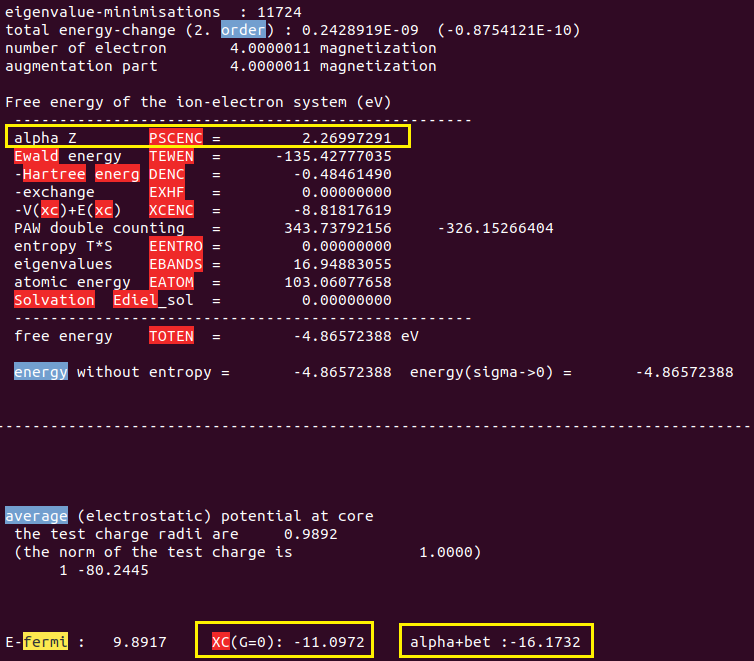
\includegraphics[height=1.85in,width=2.2in,viewport=0 0 600 495,clip]{Figures/VASP_Total_ENE.png}
\caption{\small \textrm{The Total-E calculated by VASP.}}%(与文献\cite{EPJB33-47_2003}图1对比)
\label{TOTEN_VASP}
\end{figure}
}

\section{\rm{VASP}的分波电荷密度}
\frame
{
	\frametitle{\textrm{PAW}方法的基本思想}
	\vspace{10pt}
\begin{figure}[h!]
\centering
\vspace*{-0.18in}
\includegraphics[height=1.7in,width=4.in,viewport=30 210 570 440,clip]{Figures/PAW_projector.eps}
\caption{\small \textrm{The analysis of PAW basic function.}}%(与文献\cite{EPJB33-47_2003}图1对比)
\label{PAW_baisc}
\end{figure}
{\fontsize{7.2pt}{4.2pt}\selectfont{\textcolor{red}{这里下标$i$是原子位置$\mathbf{R}_i$、原子主量子数$n$和角动量量子数$(l,m)$的缩写}}}\\
\textrm{PAW}~波函数中包含按角动量分解的原子轨道组分,因此可以在分波态密度(\textrm{PDOS})中投影出各轨道的贡献比例
}

\frame
{
	\frametitle{\textrm{PAW}方法的分波态密度}
\begin{figure}[h!]
\centering
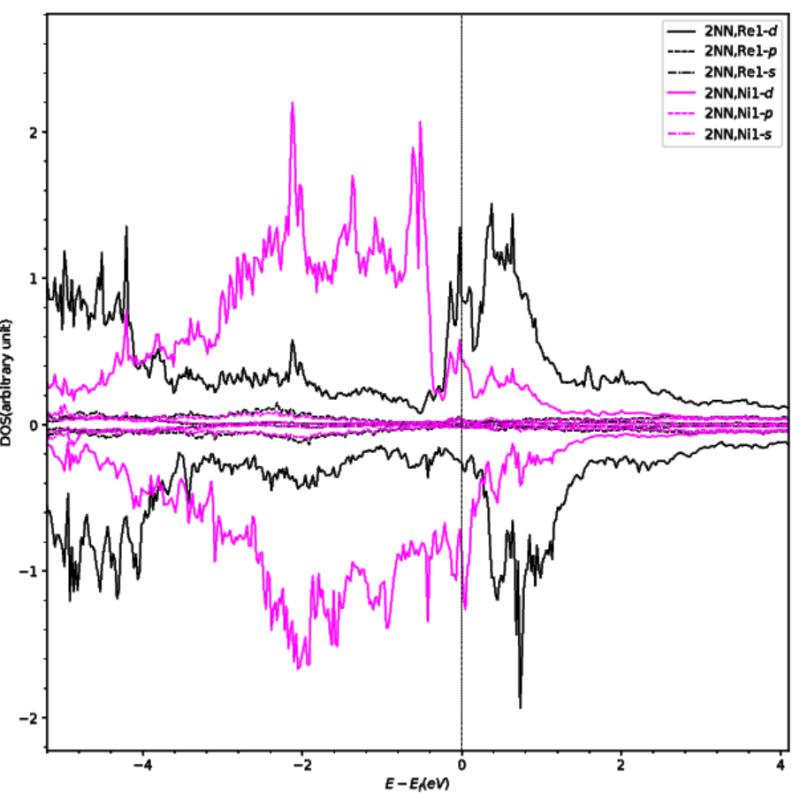
\includegraphics[height=2.5in,width=3.2in,viewport=0 0 420 400,clip]{Figures/Ni_Re-1.jpg}
\caption{\fontsize{7.2pt}{4.2pt}\selectfont{\textrm{The partial-DOS of Re and Ni.}}}%
\label{Ni-Re-DOS}
\end{figure} 
}

\frame
{
	\frametitle{\textrm{PAW}方法的分波态密度}
\begin{figure}[h!]
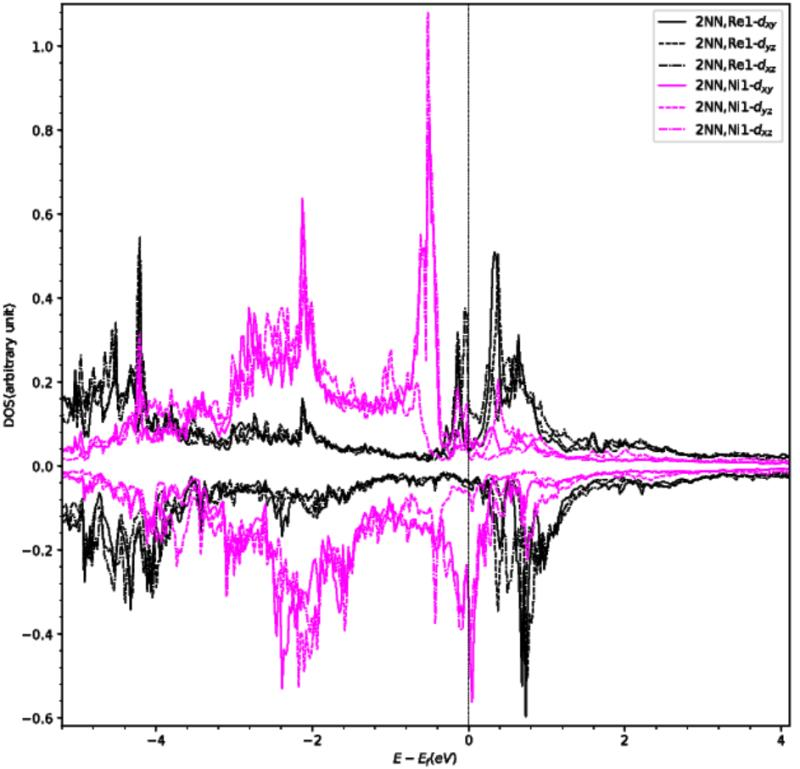
\includegraphics[height=1.7in,width=1.95in,viewport=0 0 420 400,clip]{Figures/Ni_Re-2.jpg}
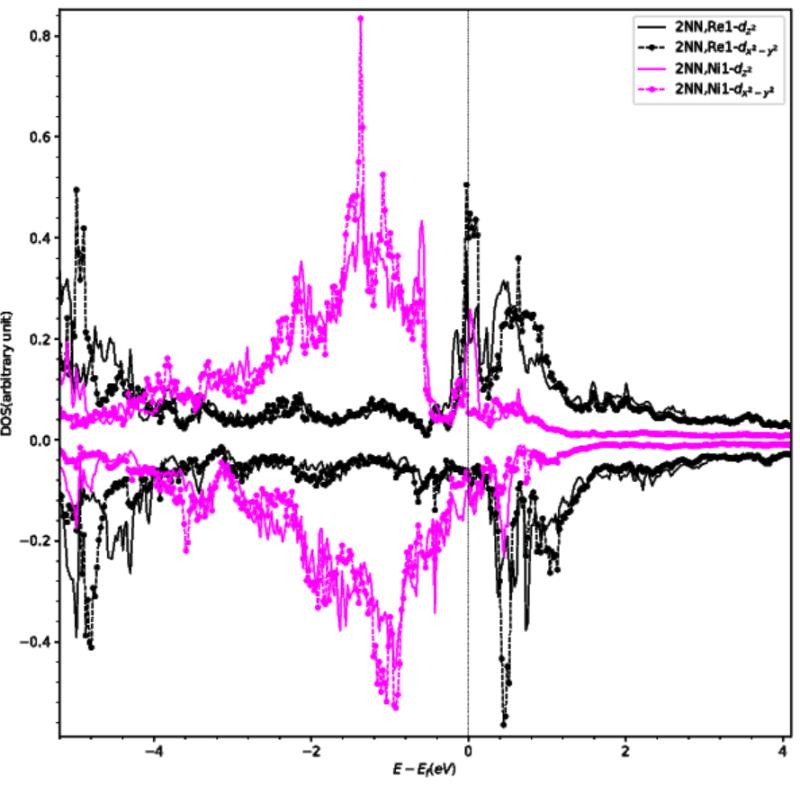
\includegraphics[height=1.7in,width=1.95in,viewport=0 0 420 400,clip]{Figures/Ni_Re-3.jpg}
\caption{\fontsize{7.2pt}{4.2pt}\selectfont{\textrm{The partial-DOS of Re and Ni $d$-orbital.}}}%
\label{Ni-Re-DOS-d}
\end{figure} 
}
%\frame
%{
%\frametitle{发展统一理论框架下的材料计算程序}
%\begin{itemize}
%	\item
%\end{itemize}
%}

\frame
{
	\frametitle{\textrm{VASP}计算的特色}
	相比于与普通的第一原理计算软件,\textrm{VASP}很好地平衡了计算效率和精度的问题,总的来说,\textrm{VASP}主要通过这几个特色保证了计算的高效能
	\begin{itemize}
	     \item 迭代与优化算法的多样性\\
		     本质上电荷密度迭代 \textrm{\&\&} 体系总能量优化是相同的优化问题,采用了类似的算法\upcite{CMS6-15_1996,PRB54-11169_1996}:\\
			\textcolor{blue}{\textrm{Pseudo-Newton、Conjugate-Gradient、Broyden~mix、damping-factor、RMM-DIIS}}
	     \item 尽可能采用局域基(原子轨道基)函数:~\\
		     \textcolor{blue}{\textrm{LREAL}}=\textcolor{red}{\textrm{.TRUE.}}\\
			优化的投影函数也尽可能在实空间表示
	     \item \textrm{PAW}原子数据集:\textcolor{blue}{优异的赝势}\upcite{PRB59-1758_1999}
	\end{itemize}
}

\frame{
	\frametitle{一维\textrm{FFT}的并行实现}
\begin{figure}[h!]
	\vspace{-0.20in}
\centering
%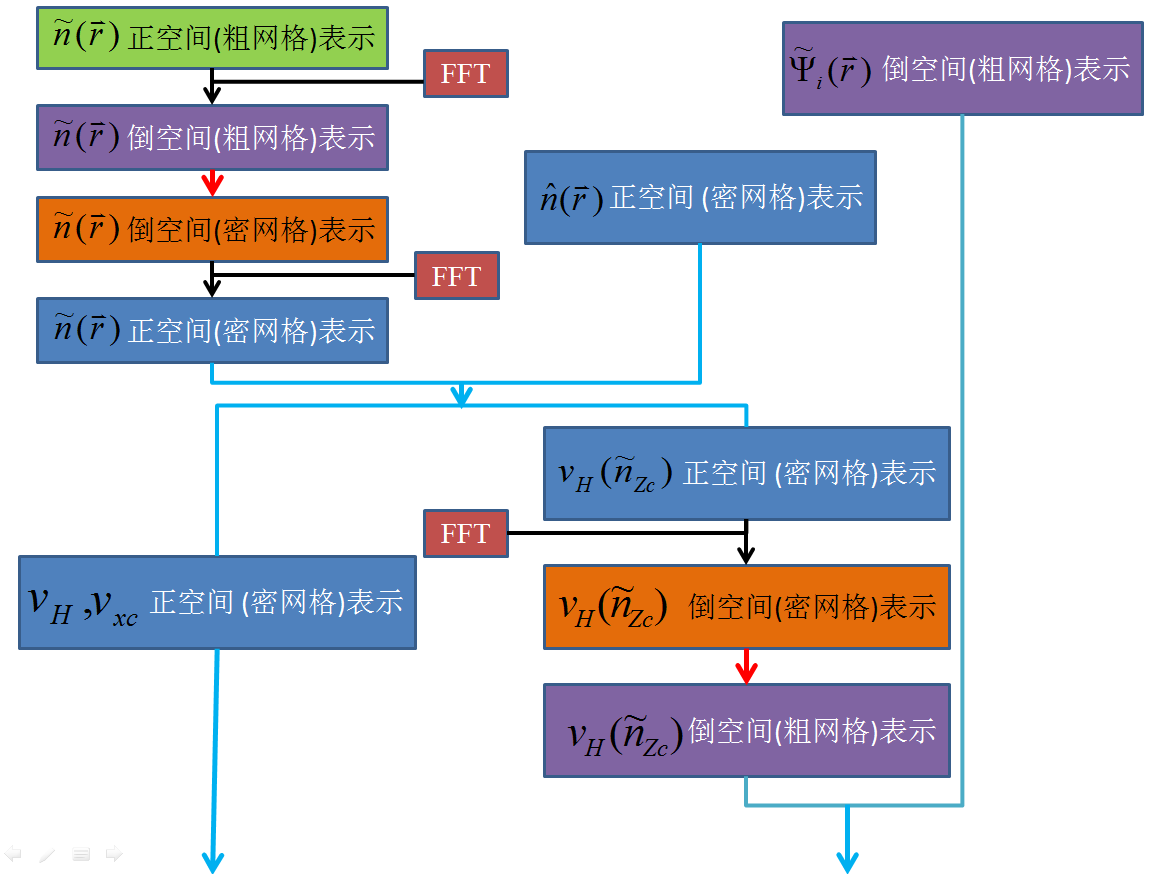
\includegraphics[height=2.7in,width=4.0in,viewport=0 0 1180 875,clip]{Figures/dual_grid.png}
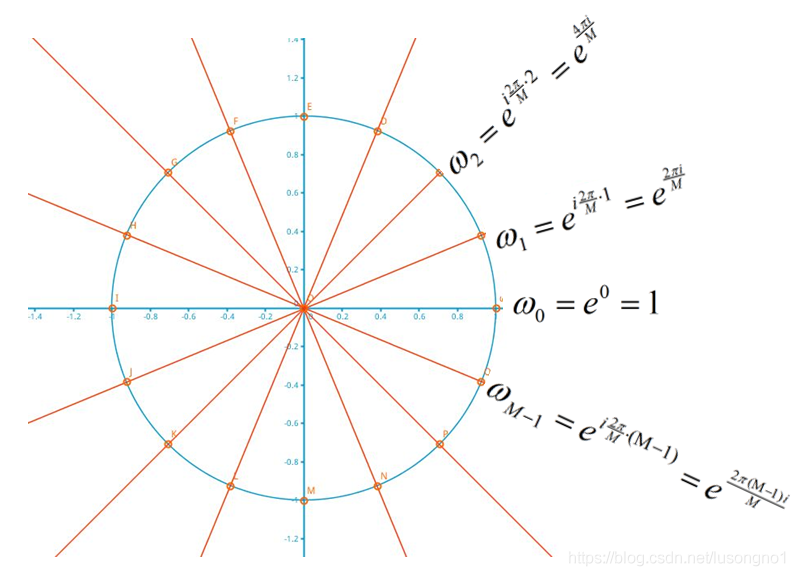
\includegraphics[height=1.6in,width=2.3in,viewport=0 10 795 570,clip]{Figures/FFT_para.png}
\vskip 0.05pt
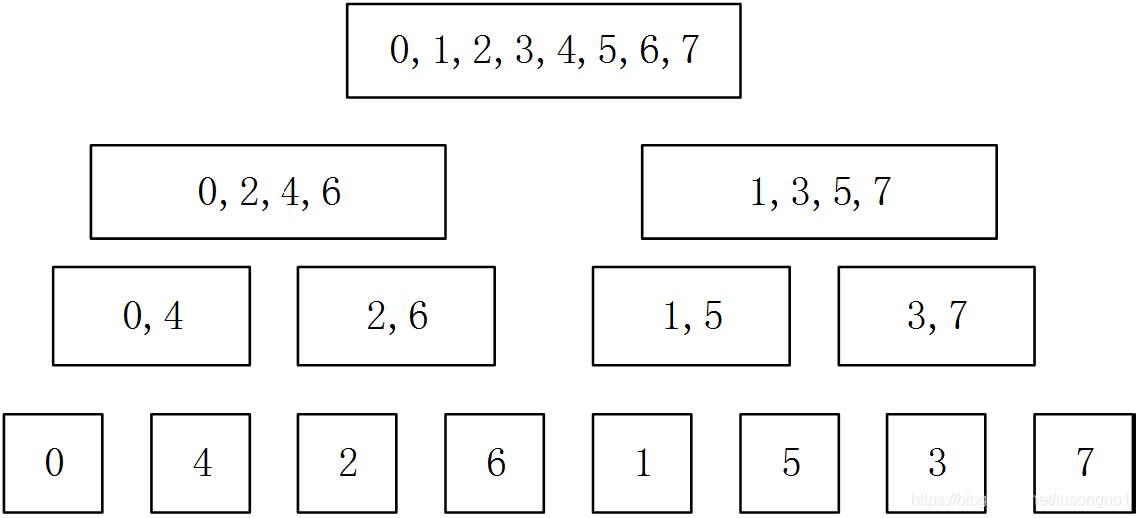
\includegraphics[height=1.1in,width=3.4in,viewport=0 0 1180 550,clip]{Figures/FFT_para-2.png}
\caption{\tiny \textrm{The Schematic description for 1D-FFT-grids in MPI.}}%(与文献\cite{EPJB33-47_2003}图1对比)
\label{1D-FFT-MPI}
\end{figure} 
}

\frame
{
	\frametitle{\textrm{VASP}计算的并行实现}
	\begin{itemize}
	     \item 中间层设计:~\textrm{FFT}网格、实空间基组与计算节点的匹配\\
		     \textcolor{magenta}{通过子程序\textrm{mgrid.F}生成中间层,实现并行负载与计算节点分配的匹配,减少\textrm{FFT}变换和实空间并行的节点间通信}
\begin{figure}[h!]
	\vspace{-0.25in}
\centering
%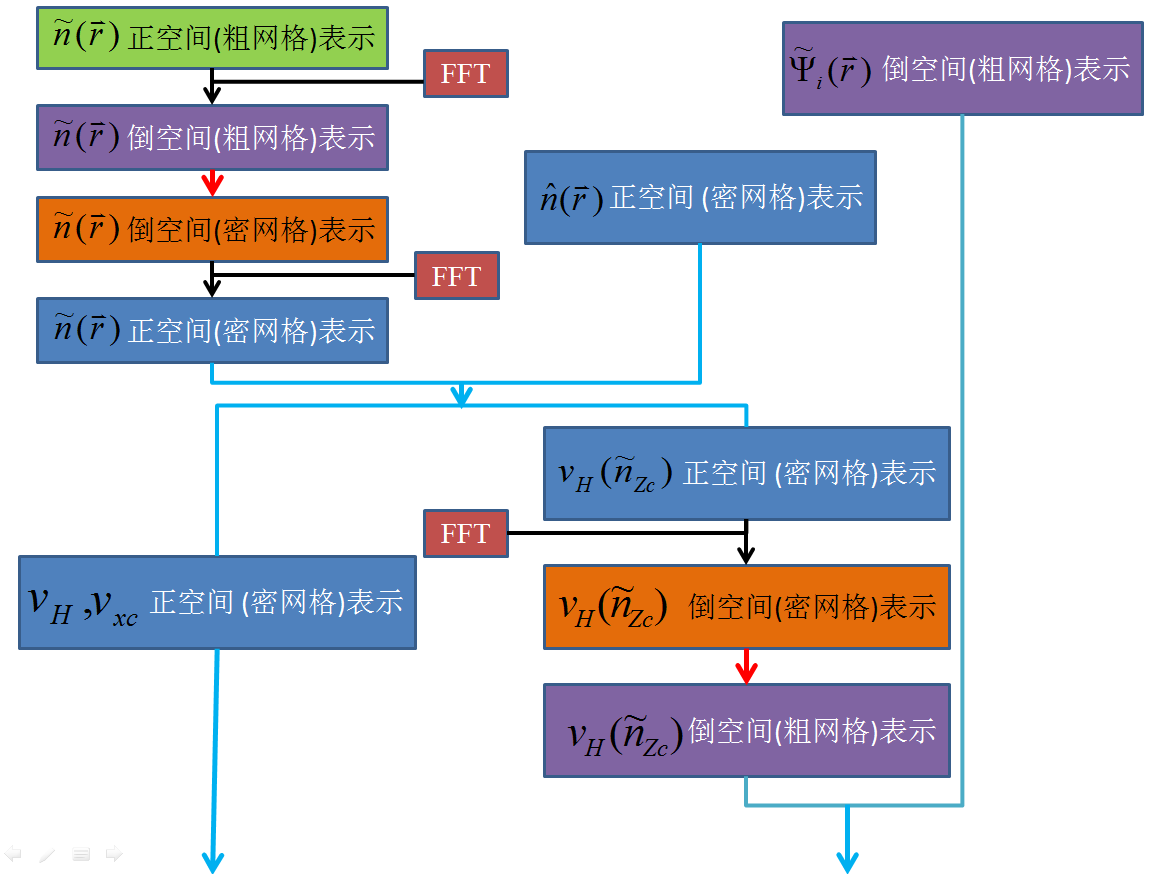
\includegraphics[height=2.7in,width=4.0in,viewport=0 0 1180 875,clip]{Figures/dual_grid.png}
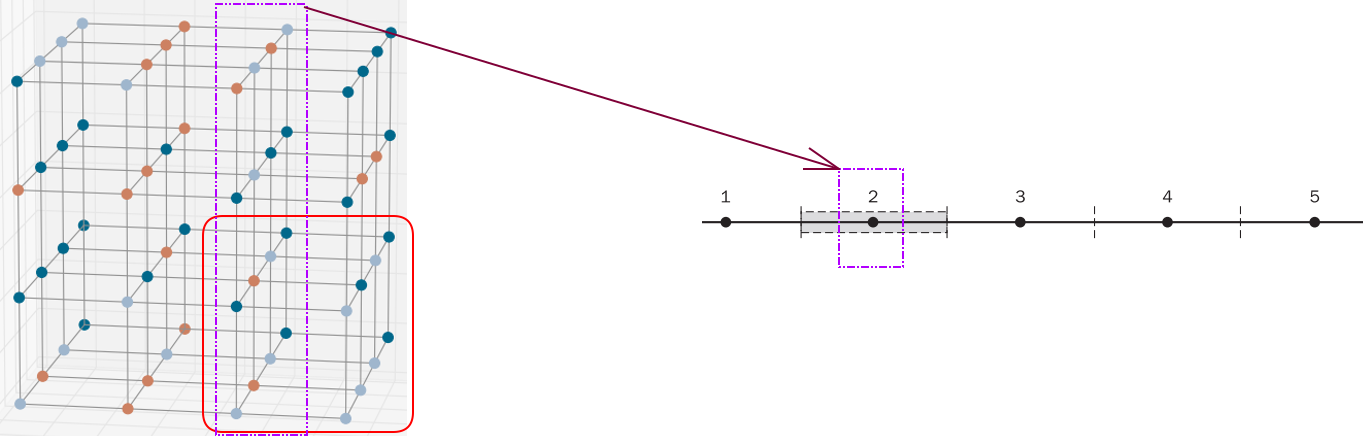
\includegraphics[height=1.0in,width=4.0in,viewport=0 0 1500 450,clip]{Figures/VASP_FFT-MPI_Reciprocal.png}
\vskip 0.5pt
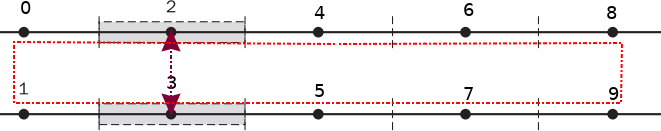
\includegraphics[height=0.7in,width=4.0in,viewport=0 0 730 150,clip]{Figures/VASP_FFT-MPI_Real.png}
\caption{\tiny \textrm{VASP:~ Reciprocal-Real space layout for grids in MPI.}}%(与文献\cite{EPJB33-47_2003}图1对比)
\label{MPI-FFT}
\end{figure} 
	\end{itemize}
}

%\appendix
%------------------------------------------------------------------------Reference----------------------------------------------------------------------------------------------
%\begin{thebibliography}{99}
%-----------------------------------------------------------------------------------------------------------------------------------------------------------------------%
%\frame
%{
%\frametitle{主要参考文献}
%{\small
%\bibitem{Singh_Book}\textrm{D. J. Singh. \textit{Plane Wave, PseudoPotential and the LAPW method} (Kluwer Academic, Boston,USA, 1994)}					%
%  \nocite{*}																				%
%}
%}
%\end{thebibliography}
\begin{thebibliography}{99}
\frame
{
\frametitle{主要参考文献}
\fontsize{7.5pt}{3.9pt}\selectfont{
        \bibitem{CMS6-15_1996}\textrm{G. Kresse and J. Furthm\"uller \textit{Comput. Mat. Sci.}, \textbf{6} (1996), 15}
	\bibitem{PRB54-11169_1996}\textrm{G. Kresse and J. Furthm\"uller \textit{Phys. Rev.} B, \textbf{54} (1996), 11169}
	\bibitem{CMS58-227_2012}\textrm{S. Curtarolo, W. Setyawan, S. Wang, J. Xue, K. Yang, R. H. Taylor, L. J. Nelson, G. L. Hart, S. Sanvito, M. Buongiorno-Nardelli, N. Mingo and O. Levy \textit{Comp. Mater. Sci.}, \textbf{58} (2012), 227}
	\bibitem{CMS97-209_2015}\textrm{S. P. Ong, S. Cholia, A. Jain, M. Brafman, D. Gunter, G. Ceder and K. A. Persson. \textit{Comp. Mater. Sci.}, \textbf{97} (2015), 209}
%	\bibitem{url_QMIP}\textrm{\url{http://www.qmip.org/qmip.org/Welcome.html}}
%	\bibitem{JPCL2-2241_2011}\textrm{J. Hachmann, R. Olivares-Amaya, S. Atahan-Evrenk, C. Amador-Bedolla, R. S. S$\acute{a}$nchez-Carrera, A. Gold-Parker, L. Vogt, A. M. Brockway and A. Aspuru-Guzik \textit{J. Phys. Chem. Lett.}, \textbf{2} (2011), 2241}
%	\bibitem{Huang_Han}黄昆\:原著、韩汝琦\:改编, {\textit{固体物理学}}\:高等教育出版社, 北京, 1988
%	\bibitem{url_Mater_Genome}\textrm{\url{https://www.whitehouse.gov/sites/default/files/microsites/ostp/materials_genome_initiative-final.pdf}}
	\bibitem{CMS49-299_2010}\textrm{W. Setyawan and S. Curtarolo \textit{Comp. Mater. Sci.}, \textbf{49} (2010), 299}
	\bibitem{CMS50-2295_2011}\textrm{A. Jain, G. Hautier, C. J. Moore, S. P. Ong, C. C. Fischer, T. M. Kristin, K. A. Persson and G. Ceder \textit{Comp. Mater. Sci.}, \textbf{50} (2011), 2295}
	\bibitem{unpublished}\textrm{D. Gunter, S. Cholia, A. Jain, M. Kocher, K. Persson, L. Ramakrishnan, S. P. Ong and G. Ceder. \textit{Community Accessible Datastore of High-Throughput Calculations: Experiences from the Materials Project} (unpublished)}
	\bibitem{Xie_Lu}谢希德、陆栋\:主编, {\textit{固体能带理论}},\:复旦大学出版社, 上海, 1998
	\bibitem{PRB59-1758_1999}\textrm{G. Kresse and D. Joubert \textit{Phys. Rev.} B, \textbf{59} (1999), 1758}
}
\nocite*{}
}
\end{thebibliography}
%{\small
%\phantomsection\addcontentsline{toc}{section}{Bibliography}	 %直接调用\addcontentsline命令可能导致超链指向不准确,一般需要在之前调用一次\phantomsection命令加以修正	%
%\bibliography{Myref}																			%
%\bibliographystyle{mybib}																		%
%  \nocite{*}																				%
%}
%-----------------------------------------------------------------------------------------------------------------------------------------------------------------------%


%-----------------------------------------------------------Beamer下不建议使用bib,因为涉及分页--------------------------------------------------------------------------%
%{\small
%\phantomsection\addcontentsline{toc}{section}{Bibliography}	 %直接调用\addcontentsline命令可能导致超链指向不准确,一般需要在之前调用一次\phantomsection命令加以修正	%
%\bibliography{Myref}																			%
%\bibliographystyle{mybib}																		%
%  \nocite{*}																				%
%}

%------------------------------------------------------------------------------------------------------------------------------------------------------------------------------%

%-------------------------------------------------------------------------Thanks------------------------------------------------------------------------------------------------
%\section{致谢}
%\frame
%{
%\frametitle{致$\quad$谢}
%\begin{itemize}
%    \setlength{\itemsep}{20pt}
%  \item 感谢本团队高兴誉、吴泉生、宋红州等各位老师参与的讨论
%  \item 感谢莫所长、宋主任以及软件中心各位老师和同事
%  \item 感谢王崇愚先生的帮助
%\end{itemize}
%}

\logo{}									%不显示logo
\frame
{
\vskip 60 pt
%%\hskip 10pt \textcolor{blue}{\Huge 感谢答辩委员会各位老师\,\textrm{!}}\\
%\vskip 35 pt
\hskip 60pt \textcolor{blue}{\Huge 谢谢大家\:!}
%%\vskip 15 pt
%%\hskip 40pt \textcolor{blue}{\Huge \textrm{for your attention\:!}}
}

%-------------------------------------------------------------------------------------------------------------------------------------------------------------------------------

\clearpage
%\end{CJK*}
\end{document}
